
\documentclass[supercite]{Experimental_Report}

\title{~~~~~~数据结构实验~~~~~~}
\author{洪炜豪}
\school{计算机科学与技术学院}
\classnum{CS2106}
\stunum{U202115512}
\instructor{周全} % 李平、孙伟平、范晔斌、陈加忠
\date{2022年6月13日}

\usepackage{algorithm, multirow}
\usepackage{algpseudocode}
\usepackage{amsmath}
\usepackage{amsthm}
\usepackage{framed}
\usepackage{mathtools}
\usepackage{subcaption}
\usepackage{xltxtra} %提供了针对XeTeX的改进并且加入了XeTeX的LOGO, 自动调用xunicode宏包(提供Unicode字符宏)
\usepackage{bm}
\usepackage{tikz}
\usepackage{tikzscale}
\usepackage{pgfplots}
\usepackage{listings}
\usepackage{graphicx}
\usepackage{float}
%\usepackage{enumerate}

\pgfplotsset{compat=1.16}

\newcommand{\cfig}[3]{
  \begin{figure}[htb]
    \centering
    \includegraphics[width=#2\textwidth]{images/#1.tikz}
    \caption{#3}
    \label{fig:#1}
  \end{figure}
}

\newcommand{\sfig}[3]{
  \begin{subfigure}[b]{#2\textwidth}
    \includegraphics[width=\textwidth]{images/#1.tikz}
    \caption{#3}
    \label{fig:#1}
  \end{subfigure}
}

\newcommand{\xfig}[3]{
  \begin{figure}[htb]
    \centering
    #3
    \caption{#2}
    \label{fig:#1}
  \end{figure}
}

\newcommand{\rfig}[1]{\autoref{fig:#1}}
\newcommand{\ralg}[1]{\autoref{alg:#1}}
\newcommand{\rthm}[1]{\autoref{thm:#1}}
\newcommand{\rlem}[1]{\autoref{lem:#1}}
\newcommand{\reqn}[1]{\autoref{eqn:#1}}
\newcommand{\rtbl}[1]{\autoref{tbl:#1}}

\algnewcommand\Null{\textsc{null }}
\algnewcommand\algorithmicinput{\textbf{Input:}}
\algnewcommand\Input{\item[\algorithmicinput]}
\algnewcommand\algorithmicoutput{\textbf{Output:}}
\algnewcommand\Output{\item[\algorithmicoutput]}
\algnewcommand\algorithmicbreak{\textbf{break}}
\algnewcommand\Break{\algorithmicbreak}
\algnewcommand\algorithmiccontinue{\textbf{continue}}
\algnewcommand\Continue{\algorithmiccontinue}
\algnewcommand{\LeftCom}[1]{\State $\triangleright$ #1}

\newtheorem{thm}{定理}[section]
\newtheorem{lem}{引理}[section]

\colorlet{shadecolor}{black!15}

\theoremstyle{definition}
\newtheorem{alg}{算法}[section]

\def\thmautorefname~#1\null{定理~#1~\null}
\def\lemautorefname~#1\null{引理~#1~\null}
\def\algautorefname~#1\null{算法~#1~\null}

\begin{document}
\begin{sloppypar}
\maketitle

\clearpage

\pagenumbering{Roman}

\tableofcontents[level=2]
\clearpage

\pagenumbering{arabic}

\section{基于顺序存储结构的线性表实现}

\subsection{问题描述}

线性表是最基本、最简单、也是最常用的一种数据结构。线性表(linear list)是数据结构的一种,一个线性表是n个具有相同特性的数据元素的有限序列。\\

顺序线性表中数据元素之间的关系是一对一的关系,即除了第一个和最后一个数据元素之外,其它数据元素都是首尾相接的。这些数据元素在物理存储中相邻。\\

在数据结构逻辑层次上细分,线性表可分为一般线性表和受限线性表。一般线性表也就是我们通常所说的“线性表”,可以自由的删除或添加结点。受限线性表主要包括栈和队列,受限表示对结点的操作受限制。\\

线性表的逻辑结构简单,便于实现和操作。因此,线性表这种数据结构在实际应用中是广泛采用的一种数据结构。\\

本实验的目的是制作一个一般线性表,并对其能够实现进行一些基本和进阶操作。\\

\subsection{系统设计}

由于顺序线性表的结构简单,使用数组即可轻松对应实现。线性表结构的声明如下:

\begin{lstlisting}[breaklines][breaklines][language=C]

typedef struct{  //顺序表(顺序结构)的定义
	ElemType * elem;
	int length;
	int listsize;
}SqList;

typedef struct{  //线性表的管理表定义
     struct { char name[30];
     		  SqList L;	
      } elem[10];
      int length;
      int listsize;
 }LISTS;
\end{lstlisting}

在系统的执行中,给出系统可执行的功能,先读取用户输入的功能编号,然后利用Switch语句判断来执行对应的功能函数。这种系统结构便于增加和删除功能,代码也更加直观,不易出错。后续实验的系统均沿用此系统结构,不再赘述。

\subsection{系统实现}

1.创建线性表

\begin{lstlisting}[breaklines][language=C]

status InitList(SqList& L)//线性表初始化 
{
	if(L.elem){
        return INFEASTABLE;
	}
	L.elem = (ElemType *)malloc( LIST_INIT_SIZE * sizeof (ElemType)); //分配初始内存
	L.length=0;//设置初始表长
	L.listsize=LIST_INIT_SIZE;//初始化元素容量
	return OK;
}

\end{lstlisting}

2.销毁线性表

\begin{lstlisting}[breaklines][language=C]

status DestroyList(SqList& L)
{
    if(!L.elem){
        return INFEASTABLE;
	}
	free (L.elem);//释放数据元素的空间
	L.elem=NULL;//指针设为空
    L.length=0;//长度置零
    L.listsize=0;
	return OK; 
}

\end{lstlisting}

3.清空线性表

\begin{lstlisting}[breaklines][language=C]

status ClearList(SqList& L)
// 如果线性表L存在,删除线性表L中的所有元素,返回OK,
否则返回INFEASIBLE。
{
    if(!L.elem){
        return INFEASTABLE;
	}
	free (L.elem);
    L.length=0;
    L.listsize=0;
	return OK; 
}

\end{lstlisting}

4.线性表判空

\begin{lstlisting}[breaklines][language=C]

status ListEmpty(SqList L)
// 如果线性表L存在,判断线性表L是否为空,空就返回TRUE,
否则返回FALSE;如果线性表L不存在,返回INFEASIBLE。
{
    if(!L.length&&L.elem){//线性表存在且为空 
        return OK;
    }
    if(L.length&&L.elem){//线性表存在且非空 
        return ERROR;
    }
    if(L.elem==NULL&&L.length==0){//线性表不存在
        return INFEASTABLE;
    }
}

\end{lstlisting}

5.求线性表长度

\begin{lstlisting}[breaklines][language=C]

status ListLength(SqList L)
// 如果线性表L存在,返回线性表L的长度,否则返回INFEASIBLE。
{
    if(L.elem){
        return L.length;
    }
    return INFEASTABLE;
}

\end{lstlisting}

6.获取线性表元素

\begin{lstlisting}[breaklines][language=C]

status GetElem(SqList L,int i,ElemType &e)
// 如果线性表L存在,获取线性表L的第i个元素,保存在e中,返回OK;如果i不合法,返回ERROR;如果线性表L不存在,返回INFEASIBLE。
{
    if(L.elem==NULL){
        return INFEASTABLE;
    }
    if(i<1||i>L.length){
        return ERROR;
    }
     //未执行上方if语句则i合法,获取元素
    e=L.elem[i-1];//逻辑位置转换为物理位置后获取元素保存在e中
    return OK;
}

\end{lstlisting}

7.查找元素

\begin{lstlisting}[breaklines][language=C]

int LocateElem(SqList L,ElemType e)
// 如果线性表L存在,查找元素e在线性表L中的位置序号并返回该序号;如果e不存在,返回0;当线性表L不存在时,返回INFEASIBLE(即-1)。
{
    if(L.elem==NULL){
        return INFEASTABLE;
    }
    int j;
    for(j=0;j<L.listsize;j++){//顺序查找线性表
        if(e==L.elem[j]){ //找到则返回
            return j+1;
        }
    }
    return 0;//遍历一遍没找到返回0
}

\end{lstlisting}

8.查找元素的前驱

\begin{lstlisting}[breaklines][language=C]

status PriorElem(SqList L,ElemType e,ElemType &pre)
// 如果线性表L存在,获取线性表L中元素e的前驱,保存在pre中,返回OK;如果没有前驱,返回ERROR;如果线性表L不存在,返回INFEASIBLE。
{
    if(L.elem==NULL){
        return INFEASTABLE;
    }
    int j;
    for(j=0;j<L.length;j++){
        if(e==L.elem[j])
		{
            if(j!=0){
            pre=L.elem[j-1];
            return OK;
			}
			else{
				return 12;//此处代表存在该元素而该元素在第一个没有前驱
			}
        }
    }
    return ERROR;
}

\end{lstlisting}

9.查找元素的后继

\begin{lstlisting}[breaklines][language=C]

status NextElem(SqList L,ElemType e,ElemType &next)
// 如果线性表L存在,获取线性表L元素e的后继,保存在next中,返回OK;如果没有后继,返回ERROR;如果线性表L不存在,返回INFEASIBLE。
{
    if(L.elem==NULL){
        return INFEASTABLE;
    }
    int j;
    for(j=0;j<L.length;j++){
        if(e==L.elem[j]){
        	if(j!=L.length-1){
        		 next=L.elem[j+1];
            return OK;
			}
           if(j==L.length-1){
           	return 13;  //此处代表存在该元素而该元素在最后一个没有后继
		   }
        }
        
    }
    return ERROR;
}
}

\end{lstlisting}

10.插入元素

\begin{lstlisting}[breaklines][language=C]

status ListInsert(SqList &L,int i,ElemType e)
// 如果线性表L存在,将元素e插入到线性表L的第i个元素之前,返回OK;当插入位置不正确时,返回ERROR;如果线性表L不存在,返回INFEASIBLE。
{
    if(L.elem==NULL){
		printf("线性表不存在!");
        return INFEASTABLE;
    }
    int i;
	if(j==0||j>L.length+1){//如果i超过表长2以上或不为正自然数,则不合法,无法找到对应的插入位置
        return ERROR;
    }
     if(L.length==0){//如果表为空线性表
        L.elem[0]=e;
        L.length++;
        return OK;
    }
    int a[100];
    for(i=0;i<L.length;i++){
        a[i]=L.elem[i];
    }
    L.length++;L.listsize++;
    L.elem=(ElemType *) malloc(sizeof(ElemType)*L.listsize);//扩容线性表
    for(i=j;i<L.length;i++){
        L.elem[i]=a[i-1];
    }
    L.elem[j-1]=e;
    for(i=0;i<j-1;i++){
        L.elem[i]=a[i];
    }
    return OK;
   

\end{lstlisting}

11.删除元素

\begin{lstlisting}[breaklines][language=C]

status ListDelete(SqList &L,int i,ElemType &e)
// 如果线性表L存在,删除线性表L的第i个元素,并保存在e中,返回OK;当删除位置不正确时,返回ERROR;如果线性表L不存在,返回INFEASIBLE。
{
    if(L.elem==NULL){
        return INFEASTABLE;
    }
    int i;
    if(j==0||j>L.length){//如果i超过表长2以上或不为正自然数,则不合法,无法找到对应的删除位置
        return ERROR;
    }
    L.length--;L.listsize--;//表长-1
    e=L.elem[j-1];//保存删除的元素到e
    for(i=j-1;i<L.length;i++){//从删除的位置开始,使其后所有元素向表头移动1
    L.elem[i]=L.elem[i+1];
        }
    return OK;

\end{lstlisting}

12.遍历输出线性表

\begin{lstlisting}[breaklines][language=C]

status ListTraverse(SqList L)
// 如果线性表L存在,依次显示线性表中的元素,每个元素间空一格,返回OK;如果线性表L不存在,返回INFEASIBLE。
{
    if(L.elem==NULL){
        return INFEASTABLE;
    }
    else{
        if(L.length==0){
        L.length++;
        return OK;
    	}
    }
    printf("\n-----------all elements -----------------------\n");
    for(int i=0;i<L.length;i++){
        if(i==0){
            printf("%d",L.elem[i]);
        }
        else{
            printf(" %d",L.elem[i]);
        }
    }
    printf("\n");
    return OK;
}

\end{lstlisting}

附加功能:

13.最大连续子数组和

\begin{lstlisting}[breaklines][language=C]

status MaxSubArray(SqList L)//最大连续子数组和
{
	 if(L.elem==NULL){
        return INFEASTABLE;
    }
    else{
        if(L.length==0){
        L.length++;
        return OK;
    	}
    }
	int thissum=0,maxsum=0,j;
	for(j=0;j<L.length;j++)//只需遍历一遍,算法复杂度O(n) ,当当前累计的值小于0,则归零重新累加 
	{
		thissum+=L.elem[j];
		if(thissum>maxsum)
			maxsum=thissum;
		else if(thissum<0)
			thissum=0;
	}
	return maxsum;
}

\end{lstlisting}

14.和为K的子数组个数 

\begin{lstlisting}[breaklines][language=C]
思想:
暴力求解
从前往后求和sum[i]为到第i项时候的和
那么sum[i:j] = sum[j]-sum[i]
遍历所有区间,用上面的公式快速求出各个区间的值,符合条件则结果+1。

status SubArrayNum(SqList L,int k)//和为K的子数组个数 
{
	if(L.elem==NULL){
        return INFEASTABLE;
    }
    else{
        if(L.length==0){
        L.length++;
        return OK;
    	}
    }
	int sum=0,i,j;
    for (i=0;i<L.length;i++)//对于每个元素,都对其与后面的所有元素进行累加,复杂度O(n^2) 
    {
        int num=0;
        for(j=i;j<L.length;j++){
            num+=L.elem[j];
            if(num==k) sum++;
        }
    }
    return sum;
}

/*哈希表算法
思想:
假如到第i个元素的时候,总和为sum[i],很显然,可以将sum[i]分为两部分:sum[i] = (sum[i]-k)+k,我们在前边已经得到的sum[x],(0<=x<i)中找到能值等于sum[i]-k的那一个,显然x+1到i部分的值就是k,这样的x有几个,那么到当前索引i的时候,就会有几个子数组和为k。

所以做法如下:
遍历nums,并且依次记录累加和sum
使用哈希表d 记录累加和出现的次数 (如果出现过+1,没出现过=1)
查询以当前元素结尾的和为k的子数组有多少个,用sum[i]-k则得到与目标k的差距,找到等于差距的累计和的个数,加到结果上
status SubArrayNum(SqList L,int k)
{
	 Map<Integer,Integer> map=new HashMap<Integer, Integer>();
        map.put(0,1);
        int count=0;
        int sum=0;
        for (int i=0;i<L.length;i++){
            sum+=L.elem[i];
            if (map.get(sum-k)!=null){
                count+=map.get(sum-k);
            }
            //如果总和没出现过,则添加进哈希表,如果出现过,哈希表中的值+1
            if(map.get(sum)==null)
                map.put(sum,1 );
            else
                map.put(sum,map.get(sum)+1 );
        }
        return count;
} 
*/

\end{lstlisting}

15.链表排序

\begin{lstlisting}[breaklines][language=C]

int cmp(const void *a, const void *b){
   ElemType *c=(ElemType*)a; ElemType *d=(ElemType*)b; 
   return *c-*d;
}
status sortList(SqList L)//链表排序
{
	if(L.elem==NULL){
        return INFEASTABLE;
    }
    else{
        if(L.length==0){
        L.length++;
        return OK;
    	}
    }
	qsort(L.elem,L.length,sizeof(L.elem[0]),cmp);//快速排序
	return OK;
}

\end{lstlisting}

16.文件读写
\begin{lstlisting}[breaklines][language=C]
status  SaveList(SqList L,char FileName[])//实现线性表的文件形式保存 
// 如果线性表L存在,将线性表L的的元素写到FileName文件中,返回OK,否则返回INFEASIBLE。
{
    if(L.elem==NULL){
        return INFEASIBLE;
    }
    FILE *fp = fopen(FileName , "w");//定义文件指针
    if (fp == NULL) //只写方式打开文件并判断打开是否成功
	{
	    puts("Fail to open file!");
	    exit(1);
	}
    for(int i=0;i<L.length;i++)  
        fprintf(fp,"%d ",L.elem[i]); 
    fclose(fp);//关闭文件 
    return OK;
}
status  LoadList(SqList &L,char FileName[])
// 如果线性表L不存在,将FileName文件中的数据读入到线性表L中,返回OK,否则返回INFEASIBLE。
{
   
    int i=0;
	if(L.elem){
        return INFEASIBLE;
    }
    FILE* fp = fopen(FileName , "r");
    if (fp == NULL)
	{
	    puts("Fail to open file!");
	    exit(1);
	}
    L.elem=(ElemType *) malloc(sizeof(ElemType)*LIST_INIT_SIZE); //为读取的线性表申请空间
    while(!feof(fp)){
    	fscanf(fp,"%d ",&L.elem[i++]); 
    	L.length++;
	}
    fclose(fp); 
    return OK;
}

\end{lstlisting}

17.多线性表操作

\begin{lstlisting}[breaklines][language=C]

typedef struct{  //线性表的管理表定义
     struct { char name[30];
     		  SqList L;	
      } elem[10];
      int length;
      int listsize;
 }LISTS;
 
void _LISTS()//多线性表操作 
{ 
	LISTS Lists;
    int n,e,op=100;
    char name[30];
    Lists.length=0;
    printf("请输入要创建的顺序表个数\n");
	scanf("%d", &n);
	while(n--)
   {
    	printf("请输入表名\n");
		scanf("%s",name);
   		AddList(Lists,name);
   		printf("输入元素,以回车结束\n");
    	do
  			{
     		scanf("%d",&e); 
			ListInsert(Lists.elem[Lists.length-1].L,Lists.elem[Lists.length-1].L.length+1,e); 
   			}while(getchar()!='\n');
   }
	printf("1.增加新表 2.移除一个线性表 3.查找线性表 4.查看全表 5.对特定表操作 0.返回上级\n");
	printf("输入您的选项\n");
	while(op){
	 	 system("cls");	printf("\n\n");
	 	printf("1.增加新表 2.移除一个线性表 3.查找线性表 4.查看全表 5.对特定表操作 0.返回上级\n");
	 	printf("输入您的选项\n");
	 	scanf("%d",&op);
	 	switch(op){
case 1:
printf("请输入要创建的顺序表个数\n");
scanf("%d", &n);
while(n--)
{
    	printf("请输入表名\n");
	scanf("%s",name);
   	AddList(Lists,name);
   	printf("输入元素,以回车结束\n");
    	do{
     	scanf("%d",&e); 			ListInsert(Lists.elem[Lists.length-1].L,Lists.elem[Lists.length-1].L.length+1,e); 
   		}while(getchar()!='\n');
    getchar();getchar();
	break;
case 2:
	printf("请输入要删除的表名\n");
	scanf("%s",name);
	if (RemoveList(Lists,name)==OK)
	   	{
   			printf("删除成功"); 
		}
   	else printf("删除失败");
   	getchar();getchar();
	break;
case 3:
	printf("请输入要查找的表名\n");
	scanf("%s",name);
	if (n=LocateList(Lists,name))
   	{
   		printf("%s ",Lists.elem[n-1].name);
   		ListTraverse(Lists.elem[n-1].L);
         putchar('\n');
   	}
   	else printf("查找失败");
   	getchar();getchar();
	break;
case 4:
	printflist(Lists);
	getchar();getchar();
	break;
case 5:
	printf("请输入要操作的表名\n");
	scanf("%s",name);
	if (n=LocateList(Lists,name))
   	{
   		__LISTS(Lists,n);//该功能为其中一个线性表做单独操作,进入三级菜单,见附录
   	}
   	else{
   		printf("该表不存在!");
		}
	getchar();getchar();
	break;
case 0:
     break;
    	default:
    	printf("输入有误,请重新输入");
    	getchar();getchar();
    		}	
		}	
  	}
}

status AddList(LISTS &Lists,char ListName[])//创建新表
{
    Lists.elem[Lists.length].L.elem = (ElemType *) malloc(LIST_INIT_SIZE  * sizeof( ElemType ));	
	if ( !Lists.elem[Lists.length].L.elem ){
		printf("存储空间申请失败\n");
		exit(OVERFLOW);
	} 
    Lists.elem[Lists.length].L.length=0;
    Lists.elem[Lists.length].L.listsize=100;
    strcpy(Lists.elem[Lists.length].name,ListName);
    Lists.length++;
}

status RemoveList(LISTS &Lists,char ListName[])
// Lists中删除一个名称为ListName的线性表
{
    int i=0;
    while(Lists.elem[i].name[0]){
        if(!strcmp(Lists.elem[i].name,ListName)){
        	strcpy(Lists.elem[i].name,"0");
            for(int j=i;j<Lists.length-1;j++){
                Lists.elem[j]=Lists.elem[j+1];
            }
            Lists.length--;
            return OK;
        }
        i++;
    }
    return FALSE;
}

int LocateList(LISTS Lists,char ListName[])
// 在Lists中查找一个名称为ListName的线性表,成功返回逻辑序号,否则返回0
{
    int i=0;
    while(Lists.elem[i].name[0]){
        if(!strcmp(Lists.elem[i].name,ListName)){
            return i+1;
        }
        i++;
    }
    return FALSE;
}

void printflist(LISTS Lists)//输出所有的线性表
{
	for(int n=0;n<Lists.length;n++)
   {
   		printf("%s ",Lists.elem[n].name);
   		ListTraverse(Lists.elem[n].L);
        putchar('\n');
   }
}
\end{lstlisting}
\subsection{系统测试}
以下的操作中,线性表的内容为:湖北 1 3 5 湖南 1 1 -2 3 4 -5 6(加入后单独操作) 

\begin{figure}[H]


    \centering
    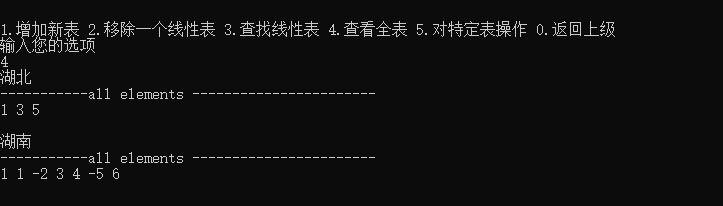
\includegraphics[width=16cm]{pic1//1.png}
    
\includegraphics[width=16cm]{pic1//2.png}
    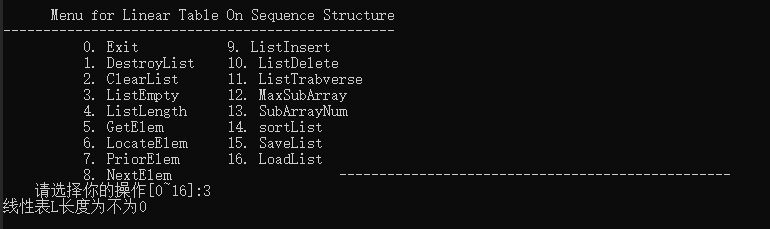
\includegraphics[width=16cm]{pic1//3.png}
    
\includegraphics[width=16cm]{pic1//4.png}
	
\includegraphics[width=16cm]{pic1//5.png}
	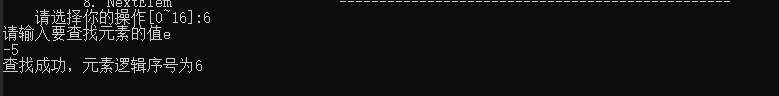
\includegraphics[width=16cm]{pic1//6.png}
	
\includegraphics[width=16cm]{pic1//7.png}
	
\includegraphics[width=16cm]{pic1//8.png}

\end{figure} 

\begin{figure}[H]
	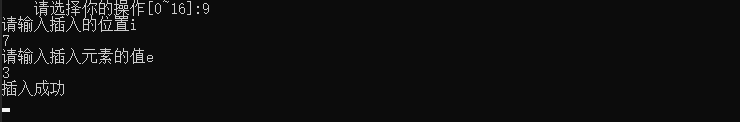
\includegraphics[width=16cm]{pic1//9.png}
	
\includegraphics[width=16cm]{pic1//10.png}
	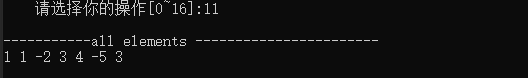
\includegraphics[width=16cm]{pic1//11.png}
	
\includegraphics[width=16cm]{pic1//12.png}
	
\includegraphics[width=16cm]{pic1//13.png}
	
\includegraphics[width=16cm]{pic1//14.png}
	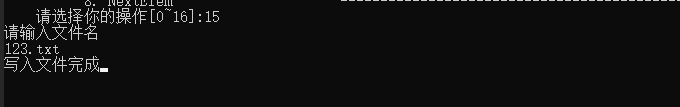
\includegraphics[width=16cm]{pic1//15.png}
	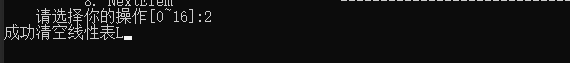
\includegraphics[width=16cm]{pic1//16.png}
	
\includegraphics[width=16cm]{pic1//17.png}
	
\includegraphics[width=16cm]{pic1//18.png}
	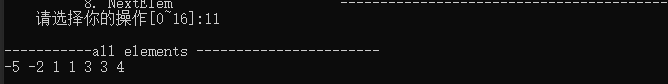
\includegraphics[width=16cm]{pic1//19.png}
\end{figure} 



\subsection{实验小结}
\begin{lstlisting}[breaklines][language=C]
本次实验的重难点有:
1.对函数及其参数的使用,包括\&符号的使用,当使用\&时,会传入参数的地址,能够改变参数本身的值;
2.对顺序线性表结构的熟练理解,确保对线性表执行的操作不产生错误或漏洞;
3.系统结构的设计,对使用进行合理的引导,令用户能够无需学习就上手,方便地使用功能;
4.多个线性表管理表的设计和能够实现对每一个线性表单独操作。
5.细节方面问题的处理:如查找后继元素分为没找到,找到了但是该元素在表尾没有后继,找到该元素且有后继三种情况,都应该说明清楚。

本次实验的心得:
1.顺序线性表的结构简单,便于操作,可以直接用角标对数据元素进行访问,较为直观。
2.顺序线性表的插入和删除操作较为复杂,时间复杂度为O(n)。
3.顺序线性表的前驱和后继可以直接通过下标加减获取,十分便利。
4.对于附加问题,学习了多种算法,
(1)对于连续子数组的最大和,有以下几种方法:
暴力破解:将给定数组的的所有子数组列出来,然后找到子数组和最大的情况,具体来说就是对数组内每一个数A[i]进行遍历,然后遍历以它们为起点的子数组,比较各个子数组的大小,找到最大连续子数组;时间复杂度O(n^2),不应该选择这样的方法。
动态规划:状态方程 : max( dp[ i ] ) = getMax( max( dp[ i -1 ] ) + arr[ i ] ,arr[ i ] )。式子的意义是:从头开始遍历数组,遍历到数组元素 arr[ i ] 时,连续的最大的和 可能为 max( dp[ i -1 ] ) + arr[ i ] ,也可能为 arr[ i ] ,做比较即可得出哪个更大,取最大值。时间复杂度为 n。
一般解法:此为我代码中的解法,对于数组array,从array[1]开始逐个进行相加,与最大值比较,并不停地更替最大值。
(2)对于和为k的子数组个数,有以下几种方法:
暴力破解:对于每个元素,都对其与后面的所有元素进行累加,再比对是否等于k,复杂度O(n^2)。
哈希表: 假如到第i个元素的时候,总和为sum[i],很显然,可以将sum[i]分为两部分:sum[i] = (sum[i]-k)+k,我们在前边已经得到的sum[x],(0<=x<i)中找到能值等于sum[i]-k的那一个,显然x+1到i部分的值就是k,这样的x有几个,那么到当前索引i的时候,就会有几个子数组和为k。
(3)对于链表排序,有以下几种方法:
快速排序:调用c库函数qsort;冒泡排序法;选择排序法等。
\end{lstlisting}

\section{基于链式存储结构的线性表实现}

\subsection{问题描述}

链式线性表具有前一实验中顺序线性表的多数特点,比如其数据元素在逻辑位置上相邻。与其不同的是,链式线性表在物理存储中并不相邻。

链式表分为单链表,循环链表和双向链表。链表可能会设置为空的头结点便于操作,也可能设置尾指针。

本实验的目的是制作一个有空头结点的单链表,并对其能够实现进行一些基本和进阶操作。

\subsection{系统设计}

链式线性表中数据元素的物理位置分开存储,这就要求使用指针来实现。对应每个数据节点,需要增加一个指向下一节点的指针,即指针域,用于串联整个线性表。因此,链式线性表的结构声明如下:

\begin{lstlisting}[breaklines][language=C]

typedef struct LNode{  //单链表(链式结构)结点的定义
      ElemType data;
      struct LNode *next;
    }LNode,*LinkList;
typedef struct LIST{  //多链表的管理表定义
     struct { char name[30];
     		  LinkList L;	
      } elem[10];
      int length;
      int listsize;
 }LISTS;

\end{lstlisting}

\subsection{系统实现}
链表的实现与顺序表具有相似性,此处概不一一举例,仅仅描述附加函数
1.链表翻转
\begin{figure}[H]
	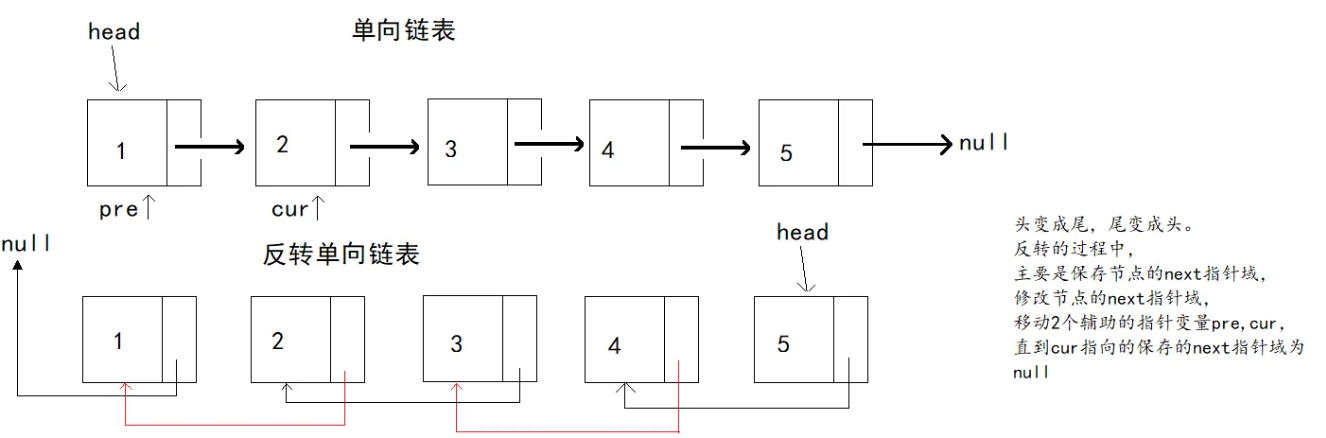
\includegraphics[width=12cm]{pic2//fanzhuan.png}
\end{figure} 
\begin{lstlisting}[breaklines][language=C]
status reverseList(LinkList L)//链表翻转
{
	if(L==NULL){
        return INFEASIBLE;
	}
	LinkList p=L->next,newHead = NULL;
    while (p != NULL) {
        LinkList remain = p->next;
        p->next = newHead;
        newHead = p;
        p = remain;
        }
    L->next=newHead;
    return OK;
}
\end{lstlisting}
2.删除链表的倒数第n个结点(这与删除链表第n个结点几乎相同)
\begin{lstlisting}[breaklines][language=C]

status RemoveNthFromEnd(LinkList L,int n,ElemType &e)//删除链表的倒数第n个结点
{
	if(L==NULL){
        return INFEASIBLE;
	}
	int length=ListLength(L);
	if(n<1||n>length) return ERROR;
	ListDelete(L,length-n+1,e);
	return OK;
}
\end{lstlisting}
3.链表排序(冒泡排序法)
\begin{figure}[H]
	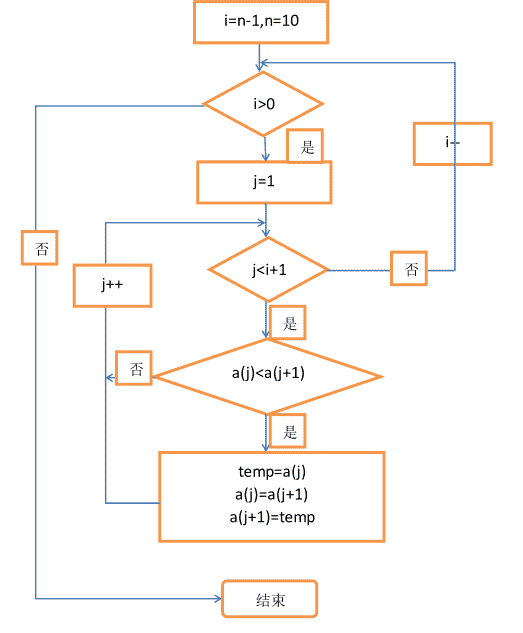
\includegraphics[width=16cm]{pic2//maopao.png}
\end{figure} 
\begin{lstlisting}[breaklines][language=C]

status sortList(LinkList L)//链表排序
{
	if(L==NULL){
        return INFEASIBLE;
	}
	struct LNode *q,*tail;
	int tmp;
	for(tail=NULL;L!=tail;tail=q){
		for(q=L;q->next!=tail;q=q->next){
			if(q->data>q->next->data&&q!=L){
				tmp=q->data;
				q->data=q->next->data;
				q->next->data=tmp;
			}
		}
	}
	return OK;	
}

\end{lstlisting}

4.文件读写

\begin{lstlisting}[breaklines][language=C]

status SaveList(LinkList L,char FileName[])
// 如果线性表L存在,将线性表L的的元素写到FileName文件中,返回OK,否则返回INFEASIBLE。
{
    if(!L){
        return INFEASIBLE;
    }
    FILE *fp;//定义文件指针
    if((fp=fopen(FileName,"w"))==NULL){
    //只写方式打开文件并判断打开是否成功
        exit(-1);
    }
    for(L=L->next;L;L=L->next){
    //顺序遍历,每次写入所访问结点的元素
        fwrite(&L->data,sizeof(ElemType),1,fp);
    }
    fclose(fp);//关闭文件
    return OK;
}

status LoadList(LinkList &L,char FileName[])
// 如果线性表L不存在,将FileName文件中的数据读入到线性表L中,返回OK,否则返回INFEASIBLE。
{
    if(L){
        return INFEASIBLE;
    }
    FILE *fp;//定义文件指针
    if((fp=fopen(FileName,"r"))==NULL){
    //只读方式打开文件并判断打开是否成功
        exit(-1);
    }
    LinkList p;//定义临时指针
    L=(LinkList)malloc(sizeof(LNode));//申请分配结点内存
    p=L;//将头指针值存储在p中
    L->next=NULL;//头结点指针域置空
    ElemType e;//定义临时元素e保存读取的元素值
    while(fread(&e,sizeof(ElemType),1,fp)){
    //一次读取一个元素,直到读取不到元素
        L->next=(LinkList)malloc(sizeof(LNode));//申请分配结点内存
        L=L->next;//L指向新结点,准备对其初始化
        L->data=e;//将读取的元素值放入新结点
        L->next=NULL;//新结点指针域置空
    }
    L=p;//L重新成为头指针
    fclose(fp);//关闭文件
    return OK;
}

\end{lstlisting}

\subsection{系统测试}
略。
\subsection{实验小结}
\begin{lstlisting}[breaklines][language=C]
本次实验的重难点有:
1.对指针的使用,要警惕和避免野指针的出现,容易访问非法内存导致程序出错。例如链表尾结点指针域不为空;
2.对链式线性表结构的熟练理解,确保对线性表执行的操作不产生错误或漏洞。例如结点的插入和删除;
3.链表头结点的使用,不能忽略其存在,也要合理利用其进行便利的数据处理。
4.多个链表管理表的设计和能够实现对每一个链表单独操作。
5.细节方面问题的处理:如查找后继元素分为没找到,找到了但是该元素在表尾没有后继,找到该元素且有后继三种情况,都应该说明清楚。
本次实验的心得:
1.链式线性表的结构虽然也较为简单,便于操作,但相对于顺序线性表复杂,需要思维的转变和习惯。它也失去了顺序表通过角标随机访问的功能。
2.链式线性表的插入和删除操作相对于顺序线性表简单,仅需对目标结点的相邻几个结点进行操作。
3.链式线性表的前驱和后继相对于顺序线性表较为复杂。
4.没有头结点时,链式线性表的前驱获取,以及插入和删除操作需要特判,故增加头结点有很多便利。
5.在进行链表排序时,掌握了冒泡排序法交换数据域和交换指针域两种方法。
交换数据域:冒泡排序,每次从第一个结点开始遍历,比较相邻两个结点的数据域。一趟下来,最大的数据域被交换到最后一个结点。接下来还从头结点起,至倒数第二个结点之间进行冒泡法排序,第二大的被交换到倒数第二个结点,每趟冒泡法排序后,尾部有序的结点增多,这些结点不需要参与下一趟冒泡排序,因此设置一个尾指针tail,它始终指向未排序结点的尾部,排序过程中指针都是和tail比较,判断是否结束循环。
交换指针域:思路与交换数据域相同,不过在成员结果较多时效率较高。
还有一种思路是先把链表的内容存放到数组中(时间为O(n)),然后,我们在对那个数组进行排序(最快为nlog(n)),最后,存放链表中(时间为O(n))。通过计算,我们可以得到它的时间复杂度为(O(nlogn))。
 
\end{lstlisting}
\begin{figure}[H]
	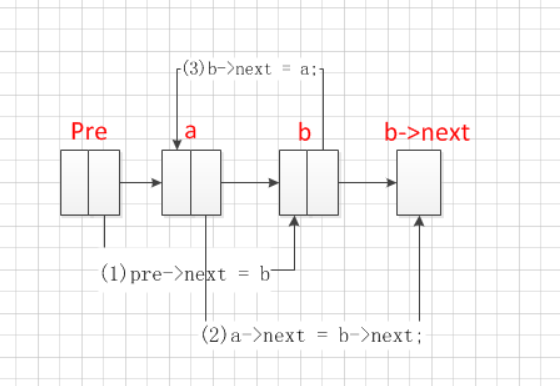
\includegraphics[width=16cm]{pic2//xianglin.png}
\end{figure}
交换指针域图示
\section{基于二叉链表的二叉树实现}

\subsection{问题描述}

二叉树(binary tree)是指树中节点的度不大于2的有序树,它是一种最简单且最重要的树。二叉树的递归定义为:二叉树是一棵空树,或者是一棵由一个根节点和两棵互不相交的,分别称作根的左子树和右子树组成的非空树;左子树和右子树又同样都是二叉树。\\
二叉树(Binary tree)是树形结构的一个重要类型。许多实际问题抽象出来的数据结构往往是二叉树形式,即使是一般的树也能简单地转换为二叉树,而且二叉树的存储结构及其算法都较为简单,因此二叉树显得特别重要。二叉树特点是每个节点最多只能有两棵子树,且有左右之分。\\
二叉树是n个有限元素的集合,该集合或者为空、或者由一个称为根(root)的元素及两个不相交的、被分别称为左子树和右子树的二叉树组成,是有序树。当集合为空时,称该二叉树为空二叉树。在二叉树中,一个元素也称作一个节点。\\
1.节点:包含一个数据元素及若干指向子树分支的信息\\
2.节点的度:一个节点拥有子树的数目称为节点的度\\
3.叶子节点:也称为终端节点,没有子树的节点或者度为零的节点\\
4.分支节点:也称为非终端节点,度不为零的节点称为非终端节点\\
5.树的度:树中所有节点的度的最大值\\
6.节点的层次:从根节点开始,假设根节点为第1层,根节点的子节点为第2层,依此类推,如果某一个节点位于第L层,则其子节点位于第L+1层\\
7.树的深度:也称为树的高度,树中所有节点的层次最大值称为树的深度\\
8.有序树:如果树中各棵子树的次序是有先后次序,则称该树为有序树\\
9.无序树:如果树中各棵子树的次序没有先后次序,则称该树为无序树\\
10.森林:由m(m≥0)棵互不相交的树构成一片森林。如果把一棵非空的树的根节点删除,则该树就变成了一片森林,森林中的树由原来根节点的各棵子树构成

\subsection{系统设计}

二叉树既可以用顺序表按层存储,也可以用二叉链表存储。本次实验中,将二叉树用二叉链表实现。将每个节点设置两个指针域,分别指向其左右孩子,即可将每个节点连接起来。最后给出根节点的指针。

\begin{lstlisting}[breaklines][language=C]

typedef struct {
         KeyType  key;
         char others[20];
	} TElemType; //二叉树结点类型定义

typedef struct BiTNode{  //二叉链表结点的定义
	      TElemType  data;
	      struct BiTNode *lchild,*rchild;
	} BiTNode, *BiTree;

typedef struct moretrees{  //多二叉树的管理表定义
     struct { char name[30];
     		  BiTree T;	
      } elem[10];
      int length;
 }BiTrees;

int front=0,rear=0;
//入队函数
void EnQueue(BiTree *a,BiTree node){
    a[rear++]=node;
}
//出队函数
BiTNode* DeQueue(BiTNode** a){
    return a[front++];
}
\end{lstlisting}

\subsection{系统实现}
0.节点访问函数,用于访问节点操作
\begin{lstlisting}[breaklines][language=C]
void visit(BiTree T)
{
    printf(" %d,%s",T->data.key,T->data.others);
}
\end{lstlisting}

1.创建二叉树

definition的输入规则:\\
二叉树带空子树的先序遍历结点序列,每个结点对应一个整型的关键字和一个字符串,当关键字为0时,表示空子树,为-1表示输入结束

\begin{lstlisting}[breaklines][language=C]


status CreateBiTree(BiTree& T, TElemType definition[],int &i)
/*根据带空枝的二叉树先根遍历序列definition构造一棵二叉树,将根节点指针赋值给T并返回OK,如果有相同的关键字,返回ERROR。*/
{
	/********** Begin *********/
	BiTree ans;
	ans = (BiTree)malloc(sizeof(BiTNode));
	T = ans;
	memset(num, 0, 1000);//num全部置0
	if (definition[0].key == 0|| definition[0].key == -1) {
		T = NULL;
		return OK;
	}//根结点为空的空二叉树
	i = 0;
	if (num[definition[i].key] == 1) return ERROR;//关键字重复
	T = (BiTree)malloc(sizeof(BiTNode));//申请节点内存
	T->data.key = definition[i].key;//数据元素赋值
	strcpy(T->data.others, definition[i].others);//数据元素赋值
	num[definition[i].key] = 1;//表示该key值已经存在,便于查重
	i++;
	if (ERROR == CreateBiTNode(T->lchild, definition, num, i) || ERROR == CreateBiTNode(T->rchild, definition, num, i))
		return ERROR;
	return OK;
	/********** End **********/
}

status CreateBiTNode(BiTree& T, TElemType definition[], int num[], int& i) {
通过递归,将definition[i]之后的数据创建为树节点
	if (definition[i].key == 0 || definition[i].key == -1) {//当前输入是结束语句或空结点,递归终止
		T = NULL;//此分支的指针域置空,代表没有孩子
		i += definition[i].key + 1;//节点计数+1
		return OK;
	}
	if (num[definition[i].key] == 1) return ERROR;//关键字重复
	T = (BiTree)malloc(sizeof(BiTNode));//申请节点内存
	T->data.key = definition[i].key;//数据元素赋值
	strcpy(T->data.others, definition[i].others);//数据元素赋值
	num[definition[i].key] = 1;
	i++;//节点计数+1
	if (ERROR == CreateBiTNode(T->lchild, definition, num, i) || ERROR == CreateBiTNode(T->rchild, definition, num, i))//创建此节点的左、右子树
		return ERROR;
	return OK;
}




\end{lstlisting}

2.销毁二叉树


\begin{lstlisting}[breaklines][language=C]
status DestroyBiTree(BiTree &T)
{
   if(!T){
			 printf("二叉树不存在!\n");
			 getchar();getchar();
			 break;
		 }   
   if (T)
   {
        DestroyBiTree(T->lchild);
        DestroyBiTree(T->rchild);
        free(T);
        T=NULL;
   }
   return OK;
}
\end{lstlisting}

3.清空二叉树

此处递归结构的构建思路是:清空一个子树,就要先清空它的左右子树,递归终止条件是一个节点没有孩子。
\begin{lstlisting}[breaklines][language=C]
status ClearBiTree(BiTree &T)
//将二叉树设置成空,并删除所有结点,释放结点空间
{
    if(!T){
			 printf("二叉树不存在!\n");
			 getchar();getchar();
			 break;
		 }    
    if(T)
    {
        ClearBiTree(T->lchild);
        ClearBiTree(T->rchild);
        free(T);
    }
    T=NULL;
    return OK;
}
\end{lstlisting}

4.二叉树判空

\begin{lstlisting}[breaklines][language=C]

status BiTreeEmpty(BiTree T)
{    
    if(T)
        return FALSE;
    else
        return TRUE;
}

\end{lstlisting}
5.二叉树深度

此处递归结构的构建思路是:求一个子树的深度,就要先求出它的左右子树的深度,取其较大者并+1,递归终止条件是一个节点是空节点,令其返回0。

\begin{lstlisting}[breaklines][language=C]

int max(int a,int b)
{
    if(a>b) return a;
    else return b;
}
int BiTreeDepth(BiTree T)
//通过递归求二叉树T的深度
{ 
    if(T==NULL) return 0; 
    else{
         return 1 + max(BiTreeDepth(T->lchild),BiTreeDepth(T->rchild));
    }
}

\end{lstlisting}

6.查找节点

此处递归结构的构建思路是:令每层递归函数返回一个指针,未查找到则返回空指针,节点对于左右节点的返回值取不为空的指针,即可最终获得查找节点的指针。

\begin{lstlisting}[breaklines][language=C]

BiTNode* LocateNode(BiTree root,KeyType value)
//查找结点
{
    if(root == NULL){
			return NULL;
		}
    else if(root != NULL && root->data.key ==value ){
			return root;
		}
    else{
			BiTree no1 = LocateNode(root->lchild,value);
			BiTree no2 = LocateNode(root->rchild,value);
			if(no1 != NULL && no1->data.key==value){
				return no1;
			}else if(no2 != NULL && no2->data.key==value){
				return no2;
			}
            else{
				return NULL ;
			}
		}
}

\end{lstlisting}

7.节点赋值

\begin{lstlisting}[breaklines][language=C]

void LocateNode1(BiTree T,KeyType e,int &i)
//检查如果进行操作,操作后是否有相同关键字
{
    if(T==NULL) return ;
    if(e==T->data.key){
        i++;//检测到相同关键字,i加1
    }
    LocateNode1(T->lchild,e,i);
    LocateNode1(T->rchild,e,i);
}

status Assign(BiTree &T,KeyType e,TElemType value)
//实现结点赋值。
{
    BiTree q;
    int i=0;//首次执行函数时进行关键字检查
	TElemType j;
    q=LocateNode(T,e);
    if(q==NULL) return ERROR;
    else {
		j=q->data;
        q->data=value;
    }//先进行赋值
    LocateNode1(T,value.key,i);//然后遍历树检查
    if(i<=1) return OK;//如果结点不重复则好赋值成功
    else{
		q->data=j;
		return 13;//如果重复则复原树,返回特定含义
	}
}

\end{lstlisting}

8.获取兄弟节点

\begin{lstlisting}[breaklines][language=C]

BiTNode* Parent(BiTree T,BiTree p)
{/*根据已知节点求父节点的核心代码*/
    if(T==NULL||T==p||p==NULL){/*T==p说明p是根节点,所有没有父节点*/
    	return NULL;
	}
	if(T->lchild==p||T->rchild==p){/*在递归过程中除根节点以外的所有节点总会先被这句代码检查一次,所以T==P只会在根节点处可能被成功触发*/
		return T;
	}
	BiTree temp;
	temp=Parent(T->lchild,p);
	if(temp!=NULL){
		return temp;
	}else{
		return Parent(T->rchild,p);
	}
}

BiTNode* GetSibling(BiTree T,KeyType e)
//实现获得兄弟结点
{
    if(T->data.key==e) return NULL;//树结点无兄弟结点
	BiTree q=LocateNode(T,e);
	BiTree T1=Parent(T,q);//找到父节点
    if(T1->lchild==q){
        return T1->rchild;
    }
   if(T1->rchild==q){
        return T1->lchild;
    }
	return NULL;
}


\end{lstlisting}

9.插入元素

\begin{lstlisting}[breaklines][language=C]

void LocateNode1(BiTree T,KeyType e,int &i)
//检查如果进行操作,操作后是否有相同关键字
{
    if(T==NULL) return ;
    if(e==T->data.key){
        i++;//检测到相同关键字,i加1
    }
    LocateNode1(T->lchild,e,i);
    LocateNode1(T->rchild,e,i);
}
status InsertNode(BiTree &T,KeyType e,int LR,TElemType c)
//插入结点,将元素为c的节点根据LR值插入关键字为e的节点的左或右孩子,LR为-1时,作为根节点插入
{
    LocateNode1(T,c.key,i);
    if(!LocateNode(T,e)){//没找到
        return ERROR;
    }
	if(i) return 13;//若插入,则存在重复元素
    if(LR==-1){//作为根节点插入的情况
        BiTree q = (BiTree)malloc(sizeof(BiTNode));
        q->lchild=NULL;
        q->rchild=T;
        q->data=c;
        T=q;
        return OK;
    }
    else{
        BiTree p=LocateNode(T,e);
        BiTree p1 = (BiTree)malloc(sizeof(BiTNode));
        p1->data=c;
        if(LR==0){//作为左子树插入,原子树作为新节点的右子树
            p1->rchild=p->lchild;
            p1->lchild=NULL;
            p->lchild=p1;
            return OK;
        }
        if(LR==1){//作为右子树插入,原子树作为新节点的右子树
            p1->rchild=p->rchild;
            p1->lchild=NULL;
            p->rchild=p1;
            return OK;
        }
    }
	return 0;
}

\end{lstlisting}

10.删除节点
功能说明:e是和T中结点关键字类型相同的给定值。删除T中关键字为e的结点;同时,根据该被删结点的度进行讨论:  

如关键字为e的结点度为0,删除即可;\\
如关键字为e的结点度为1,用关键字为e的结点孩子代替被删除的e位置;\\
如关键字为e的结点度为2,用e的左子树(简称为LC)代替被删除的e位置,将e的右子树(简称为RC)作为LC中最右节点的右子树。
\begin{lstlisting}[breaklines][language=C]

BiTNode* LocateNode2(BiTree T,KeyType e,KeyType &k)
//查找父结点
{
   BiTree q=LocateNode(T,e);
    if(T->lchild==q){
        k=1;
        return T;
    }
    if(T->rchild==q){
        k=2;
        return T;
    }
   if(T->lchild!=q&&T->rchild!=q){
   LocateNode2(T->lchild,e,k);
   LocateNode2(T->rchild,e,k);
   }
   return NULL;
}

status DeleteNode(BiTree &T,KeyType e)
//删除结点
{
    BiTree q1=T;
    int k;
    if(!LocateNode(T,e)){
        return ERROR;
    }
    if(T->data.key==e){//被删除结点为根节点的情况
        if(T->lchild==NULL&&T->rchild==NULL){
           T=NULL;
        }
        if(T->lchild&&T->rchild==NULL){
            T=T->lchild;
            free(q1);
        }
        if(T->rchild&&T->lchild==NULL){
            T=T->rchild;
            free(q1);
        }
        if(T->rchild&&T->lchild){
           BiTree q=T->lchild;
           while(q){//找到左子树的最右节点
               if(q->rchild){
                   q=q->rchild;
               }
               if(q->rchild==NULL&&q->lchild){
                   q=q->lchild;
               }
               if(q->rchild==NULL&&q->lchild==NULL){
                   break;
               }
           }
           q->rchild=T->rchild;
           T=T->lchild;
           free(q1);
        }
        return OK;
    }
    else{//被删除结点不是根节点的情况
       BiTree p=LocateNode(T,e);
       BiTree p1=LocateNode2(T,e,k);
	    BiTree p2=Parent(T,p);
         if(p->lchild==NULL&&p->rchild==NULL){//度为0
         if(k==1) p2->lchild=NULL;
         if(k==2) p2->rchild=NULL; 
       }
       if(p->lchild&&p->rchild==NULL){//度为1
         if(k==1) p1->lchild=p->lchild;
         if(k==2) p1->rchild=p->lchild;
          free(p);
       }
       if(p->rchild&&p->lchild==NULL){//度为1
         if(k==1) p1->lchild=p->rchild;
         if(k==2) p1->rchild=p->rchild;
          free(p);
       }
       if(p->rchild&&p->lchild){//度为2
           BiTree p2=T->lchild;
           while(p2){//找到左子树的最右节点
               if(p2->rchild){
                   p2=p2->rchild;
               }
               if(p2->rchild==NULL&&p2->lchild){
                   p2=p2->lchild;
               }
               if(p2->rchild==NULL&&p2->lchild==NULL){
                   break;
               }
           }
           p2->rchild=p->rchild;
           if(k==1) p1->lchild=p->lchild;
           if(k==2) p1->rchild=p->lchild;
          free(p);
       }
       return OK;
    }
}

\end{lstlisting}

11.先序遍历(用栈的非递归遍历)

\begin{lstlisting}[breaklines][language=C]

void PreOrderTraverse(BiTree T,void (*visit)(BiTree))
{
	BiTree p=T;
	stack <BiTree> s;	
    while (p || !s.empty())				//设置循环并以p和栈都为空时为结束循环标志;
	{
		if (p) {						//如果p不是空;
			visit(p);
			s.push(p);					//把p结点入栈,为的是保存p结点的右子树的位置;
			p = p->lchild;				//访问p结点的左子树;
		}
		else {
			p = s.top()->rchild;		//如果p为空,说明上个结点的左子树是空的,此时需要访问上个节点的右子树;
			s.pop();					//弹出栈顶元素,即上个节点;
		}
	}
}

\end{lstlisting}

12.中序遍历

\begin{lstlisting}[breaklines][language=C]

status InOrderTraverse(BiTree T,void (*visit)(BiTree))
//使用递归中序遍历二叉树T
{
    if (T)
    {
        InOrderTraverse(T->lchild,visit);//中序遍历左子树
        visit(T);//访问此节点
        InOrderTraverse(T->rchild,visit);//中序遍历右子树
    }
}

\end{lstlisting}

13.后序遍历

\begin{lstlisting}[breaklines][language=C]

void PostOrderTraverse(BiTree T,void (*visit)(BiTree))
//后序遍历二叉树T
{
    if (T)
    {
        PostOrderTraverse(T->lchild,visit);//后序遍历左子树
        PostOrderTraverse(T->rchild,visit);//后序遍历右子树
        visit(T);//访问此节点
    }
}

\end{lstlisting}

14.按层遍历

\begin{lstlisting}[breaklines][language=C]

int front=0,rear=0;
//入队函数
void EnQueue(BiTree *a,BiTree node){
    a[rear++]=node;
}
//出队函数
BiTNode* DeQueue(BiTNode** a){
    return a[front++];
}
void LevelOrderTraverse(BiTree T,void (*visit)(BiTree))
//按层遍历二叉树T
{
	BiTNode * p;
    //采用顺序队列,初始化创建队列数组
    BiTree a[20];
    //根结点入队
    EnQueue(a, T);
    //当队头和队尾相等时,表示队列为空
    while(front<rear) {
        //队头结点出队
        p=DeQueue(a);
        visit(p);
        //将队头结点的左右孩子依次入队
        if (p->lchild!=NULL) {
            EnQueue(a, p->lchild);
        }
        if (p->rchild!=NULL) {
            EnQueue(a, p->rchild);
        }
    }
}

\end{lstlisting}

附加功能\\
15.最大路径和

\begin{lstlisting}[breaklines][language=C]

int MaxPathSum(int& self,BiTree root,int Sum)
{
	if (root == NULL) return self;
    if ((root->lchild != NULL) && (root->rchild != NULL)){
			MaxPathSum(self,root->lchild, Sum + root->data.key);
            MaxPathSum(self,root->rchild, Sum + root->data.key);
		}           
    else if ((root->lchild != NULL) && (root->rchild == NULL))
            MaxPathSum(self,root->lchild, Sum + root->data.key);
    else if ((root->lchild == NULL) &&(root->rchild != NULL))
            MaxPathSum(self,root->rchild, Sum + root->data.key);
	else{
			if ((Sum + root->data.key) > self)
                self = Sum + root->data.key;//更新最大值
		} 
	return OK;    
}

\end{lstlisting}

16.最近公共祖先

\begin{lstlisting}[breaklines][language=C]

//使用递归查找 , 如果有一个节点与根节点匹配 , 那么直接返回根节点 , 否则依次在左子树和右子树中查找 ,
//并且用left和right分别记录左子树的返回值和右子树的返回值 , 如果节点都存在左子树中 , 那么right就一
//定为NULL , 只需要返回 left , 如果节点都存在右子树中那么直接返回 right , 如果left和right都为空 返回NULL ;
BiTNode* LowestCommonAncestor(BiTree T,KeyType e1,KeyType e2)
{
	struct BiTNode* left = NULL;
    struct BiTNode* right = NULL;
	struct BiTNode* p=LocateNode(T,e1);
	struct BiTNode* q=LocateNode(T,e2);
    if(T == NULL)
    {
        return NULL;
    }
    if(p == T || q == T)
    {
        return T;
    }

    left = LowestCommonAncestor(T->lchild, e1, e2);
    right = LowestCommonAncestor(T->rchild, e1, e2);

    if(NULL == left)
    {
        return right;
    }
    if(NULL == right)
    {
        return left;
    }
    return T;
}

\end{lstlisting}

17.翻转二叉树

\begin{lstlisting}[breaklines][language=C]

void InvertTree(BiTree &T)
{//递归交换每个结点的左右指针
	if(T==NULL) return ;
	BiTree p=T->lchild;
	T->lchild=T->rchild;
	T->rchild=p;
	InvertTree(T->lchild);
	InvertTree(T->rchild);
}

\end{lstlisting}

18.文件读写

文件读写的思路,是将二叉树的信息转换成definition的格式写入文件中,之后读取文件时,只需调用创建二叉树的函数即可,更为便利,文件写入时的思路与先序遍历一致,但要考虑空节点。读入文件后,在definition最后补入-1的关键字作为终止标识。
\begin{lstlisting}[breaklines][language=C]

status SaveBiTree(BiTree T, char FileName[])
//将二叉树的结点数据写入到文件FileName中
{
	FILE* fp;
	if ((fp = fopen(FileName, "w+")) == NULL) {
		printf("File open erroe\n ");
		return ERROR;
	};//文件写入失败
	BiTNode* stack[100], * now = T;
	int top = 0;
	stack[0] = (BiTNode*)malloc(sizeof(BiTNode));
	stack[0]->lchild = stack[0]->rchild = NULL;
	while (top > 0 || now) {//输出带空结点的二叉树前序遍历序列
		if (now) {
			fprintf(fp, "%d %s ", now->data.key, now->data.others);
			top++;
			stack[top] = now;
			now = now->lchild;
		}
		else {
			fprintf(fp, "0 null ");
			now = stack[top--]->rchild;
		}
	}//while
	fprintf(fp, "0 null -1 null ");
	fclose(fp);
	return OK;
}
status LoadBiTree(BiTree& T, char FileName[])
//读入文件FileName的结点数据,创建二叉树
{
	if (NULL != T) return INFEASIBLE;
	FILE* fp;
	if ((fp = fopen(FileName, "r+")) == NULL) {
		printf("File open erroe\n ");
		exit(-1);
	};//文件打开失败
	TElemType definition[100];
	int q = 0;
	do {//将带空结点的二叉树前序遍历序列存进definition
		fscanf(fp, "%d %s ", &definition[q].key, definition[q].others);
	} while (definition[q++].key != -1);
	fclose(fp);
	if (OK == CreateBiTree(T, definition,i))//创建二叉树
		return OK;
	return 0;
}

\end{lstlisting}

19.多二叉树管理

\begin{lstlisting}[breaklines][language=C]
以线性表形式实现多二叉树管理,与前两个实验相同。
void BITREES()//多二叉树操作 
{ 
	BiTrees Lists;
	TElemType definition[100];
    int n,e,op=100,ans,i;
    char name[30];
    Lists.length=0;
    printf("请输入要创建的二叉树个数\n");
	scanf("%d", &n);
	while(n--)
   {
    	i=0;
		printf("请输入二叉树名字\n");
		scanf("%s",name);
   		AddBiTree(Lists,name);
   		printf("以前序遍历输入二叉树各结点数据,以“-1 null“结束\n");
		do {
		    scanf("%d %s",&definition[i].key,definition[i].others);
			} while (definition[i++].key!=-1);
    	ans=CreateBiTree(Lists.elem[Lists.length-1].T,definition,i);
		 if (ans==OK){
  			  printf("二叉树创建成功!\n");
			}
		 else if(ans==ERROR){
			  printf("关键字不唯一!创建失败!\n");
			  RemoveBiTree(Lists,name);
		 }
		 memset(definition,0,100);
		 getchar();getchar();
   }
	printf("1.增加新二叉树 2.移除一棵二叉树 3.查找二叉树 4.前中后序遍历全二叉树 5.对特定树操作 0.返回上级\n");
	printf("输入您的选项\n");
while(op){
	 system("cls");	printf("\n\n");
	 printf("1.增加新二叉树 2.移除一棵二叉树 3.查找二叉树 4.前中后序遍历全二叉树 5.对特定树操作 0.返回上级\n");
	 printf("输入您的选项\n");
	 scanf("%d",&op);
switch(op){
case 1:
	printf("请输入要创建的二叉树个数\n");
	scanf("%d", &n);
	while(n--)
  	{
    	i=0;
	printf("请输入二叉树名字\n");
	scanf("%s",name);
   	AddBiTree(Lists,name);
   	printf("以前序遍历输入二叉树各结点数据,以“-1 null“结束\n");
	do {
		scanf("%d %s",&definition[i].key,definition[i].others);
		} while (definition[i++].key!=-1);
   	ans=CreateBiTree(Lists.elem[Lists.length-1].T,definition,i);
	if (ans==OK){
  		 printf("二叉树创建成功!\n");
		}
	else if(ans==ERROR){
    printf("关键字不唯一!创建失败!\n");
	RemoveBiTree(Lists,name);
		}
	memset(definition,0,100);
	getchar();getchar();
 	}
  	getchar();getchar();
	break;
case 2:
	printf("请输入要删除的二叉树名字\n");
	scanf("%s",name);
	if (RemoveBiTree(Lists,name)==OK) printf("删除成功"); 
   	else printf("删除失败");
   	getchar();getchar();
	break;
case 3:
	printf("请输入要查找的二叉树名字\n");
	scanf("%s",name);
	if (n=LocateBiTree(Lists,name))
   	{
   	printf("%s",Lists.elem[n-1].name);
	putchar('\n');
   	PreOrderTraverse(Lists.elem[n-1].T,visit);
	putchar('\n');
	InOrderTraverse(Lists.elem[n-1].T,visit);
	putchar('\n');
	PostOrderTraverse(Lists.elem[n-1].T,visit);
    putchar('\n');
   	}
    else printf("查找失败");
   	getchar();getchar();
	break;
case 4:
	printfBiTrees(Lists);
	getchar();getchar();
	break;
case 5:
	printf("请输入要操作的二叉树名字\n");
	scanf("%s",name);
	if (n=LocateBiTree(Lists,name))
   	{
   		_BITREES(Lists,n-1);//此处为对特定树操作
   	}
   	else{
   		printf("该表不存在!");
		  }
	getchar();getchar();
	break;
case 0:
    break;
default:
    	printf("输入有误,请重新输入");	
		}	
  	}
}

status AddBiTree(BiTrees &Lists,char ListName[])
{
    strcpy(Lists.elem[Lists.length].name,ListName);
    Lists.length++;
	return OK;
}

status RemoveBiTree(BiTrees &Lists,char ListName[])
// Lists中删除一个名称为ListName的二叉树
{
    int i=0;
    while(Lists.elem[i].name[0]){
        if(!strcmp(Lists.elem[i].name,ListName)){
        	strcpy(Lists.elem[i].name,"0");
            for(int j=i;j<Lists.length-1;j++){
                Lists.elem[j]=Lists.elem[j+1];
            }
            Lists.length--;
            return OK;
        }
        i++;
    }
    return FALSE;
}

int LocateBiTree(BiTrees Lists,char ListName[])
// 在Lists中查找一个名称为ListName的二叉树,成功返回逻辑序号,否则返回0
{
    int i=0;
    while(Lists.elem[i].name[0]){
        if(!strcmp(Lists.elem[i].name,ListName)){
            return i+1;
        }
        i++;
    }
    return FALSE;
}

void printfBiTrees(BiTrees Lists)
{
	for(int n=0;n<Lists.length;n++)
   {
   		printf("%s",Lists.elem[n].name);
		putchar('\n');
   		PreOrderTraverse(Lists.elem[n].T,visit);
		putchar('\n');
		InOrderTraverse(Lists.elem[n].T,visit);
		putchar('\n');
		PostOrderTraverse(Lists.elem[n].T,visit);
        putchar('\n');
   }
}

\end{lstlisting}

\subsection{系统测试}
\begin{lstlisting}[breaklines][language=C]
输入数据:
//湖南 1 a 2 b 0 null 0 null 3 c 4 d 0 null 0 null 5 e 0 null 0 null -1 null
//湖北 1 a 2 b 3 c 0 null 0 null 0 null 0 null -1 null
其中对湖南表进行特定操作,先将5e改为6e,然后在3c的右子树插入5e,再删除6e,二叉树会与初始相同,过程如下:
\end{lstlisting}
\begin{figure}[H]


    \centering
    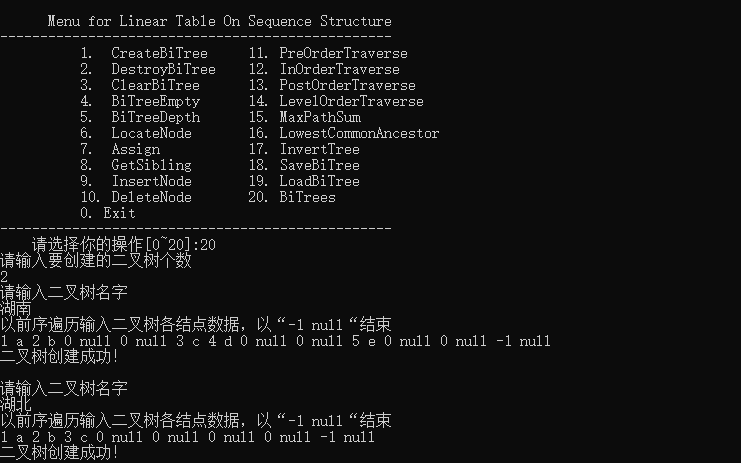
\includegraphics[width=16cm]{pic3//1.png}
    
\includegraphics[width=16cm]{pic3//2.png}
    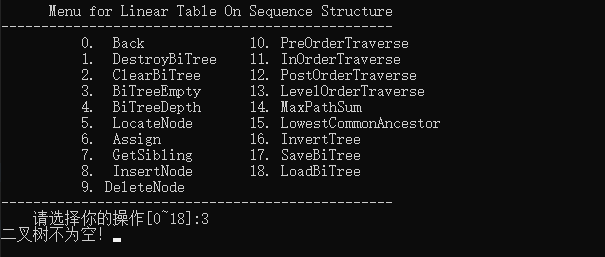
\includegraphics[width=16cm]{pic3//3.png}
    
\includegraphics[width=16cm]{pic3//4.png}
\end{figure} 

\begin{figure}[H]
	
\includegraphics[width=16cm]{pic3//5.png}
	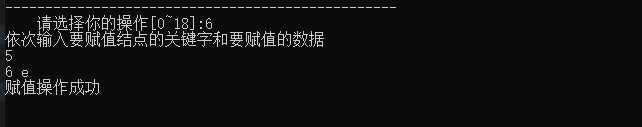
\includegraphics[width=16cm]{pic3//6.png}
	
\includegraphics[width=16cm]{pic3//7.png}
	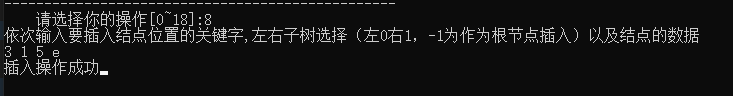
\includegraphics[width=16cm]{pic3//8.png}
	
\includegraphics[width=16cm]{pic3//9.png}
	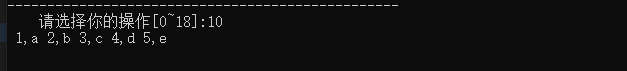
\includegraphics[width=16cm]{pic3//10.png}
	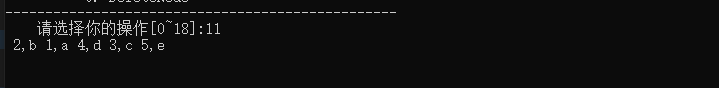
\includegraphics[width=16cm]{pic3//11.png}
	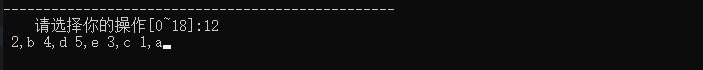
\includegraphics[width=16cm]{pic3//12.png}
	
\includegraphics[width=16cm]{pic3//13.png}
	
\includegraphics[width=16cm]{pic3//14.png}

\end{figure} 

\begin{figure}[H]
	
\includegraphics[width=16cm]{pic3//15.png}
	
\includegraphics[width=16cm]{pic3//16.png}
	
\includegraphics[width=16cm]{pic3//17.png}
	
\includegraphics[width=16cm]{pic3//18.png}
	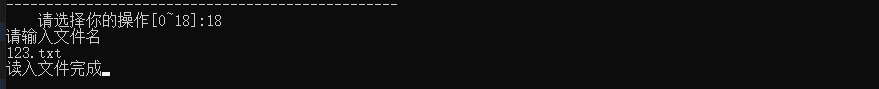
\includegraphics[width=16cm]{pic3//19.png}
	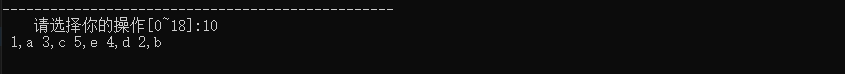
\includegraphics[width=16cm]{pic3//20.png}
\end{figure} 

\subsection{实验小结}
\begin{lstlisting}[breaklines][language=C]

本次实验的重难点有:
1.对指针的使用,要警惕和避免野指针的出现,容易访问非法内存导致程序出错。例如叶子节点指针域不为空;
2.对二叉树结构的熟练理解,确保对线性表执行的操作不产生错误或漏洞。例如节点的插入和删除;
3.对递归的使用,重在想要达到的效果而不是过程,要清楚地设置跳出递归的时机。
4.对栈和队列的使用。用于保存需要记录的数据。
4.多个二叉树管理表的设计和能够实现对每一个二叉树单独操作。
5.细节方面问题的处理:如,修改结点的值时,查无该结点和找到该结点但修改后的key发生了重复两种情况都应该说明清楚。
6.系统结构的设计,对使用进行合理的引导,令用户能够无需学习就上手,方便地使用功能;
本次实验的心得:
1.二叉树的结构相对于线性表更为复杂,同时涉及到了递归,栈和队列的使用,对知识和技能的掌握有更高的要求。
2.二叉树的插入和删除操作较为复杂,为了不造成数据的损失,需要对操作后的子树进行分类讨论和处理。
3.在做附加问题的最大路径和时,我还思考了从树中任意节点出发到任意节点的路径最大值,从而对dfs有了更加深度的理解。核心思想为递归地计算根节点左右子树的最大路径和,看是否大于0。伪代码如下:
int dfs(TreeNode root) {
        int max=0;
        if (root == NULL)
            return 0;
        int left_val = max(dfs(root->left), 0);
        int right_val = max(dfs(root->right), 0);
        max = max(root.val + left_val + right_val, max);
        return root.val + max(left_val, right_val);
    }
}
4.在做附加问题的最近公共祖先时,我不仅掌握了递归的查找方法,还掌握了用栈的方法。

\end{lstlisting}

\section{课程的收获和建议}

在本课程中,我学习了各种数据在计算机中的存储结构,理清了逻辑结构和物理结构的关系,掌握了对特定结构中存储的数据元素的各种操作,对计算机中数据的存储有了更加深刻的认识。

对本课程的建议是,希望能够有更多更方便地和老师交流与答疑的机会,能够在细节上查漏补缺。最后两个实验的时间稍显紧迫,可以适当调整课程开始时间。
学习了LaTeX的使用,真是受益匪浅呢(笑)。
\appendix
\section{附录 参考文献}
\begin{lstlisting}[breaklines][language=C]
[1]  卢萍,李开,王多强,甘早斌. C语言程序设计,北京:清华大学出版社,2019
[2]  [美]马克·艾伦·维斯. 数据结构与算法分析(C语言描述)第二版,机械工业出版社出版社
\end{lstlisting}


\section{附录 基于顺序存储结构线性表实现的源程序}

\begin{lstlisting}[breaklines][language=C]

#include<stdio.h>
#include<malloc.h>
#include<stdlib.h>
#include<string.h>

typedef int status; 
typedef int ElemType; 

#define TRUE 1
#define FALSE 0
#define OK 1
#define ERROR 0
#define INFEASTABLE -1
#define INFEASIBLE -1
#define OVERFLOW -2

#define LIST_INIT_SIZE 100
#define LISTINCREMENT  10
typedef struct{  
	ElemType *elem;
	int length;
	int listsize;
}SqList;
typedef struct{  //线性表的管理表定义
     struct { char name[30];
     		  SqList L;	
      } elem[10];
      int length;
      int listsize;
 }LISTS;

int cmp(const void *a, const void *b){
   ElemType *c=(ElemType*)a; ElemType *d=(ElemType*)b; 
   return *c-*d;
}

status InitList(SqList& L);
status DestroyList(SqList& L);
status ClearList(SqList& L);
status ListEmpty(SqList L);
status ListLength(SqList L);
status GetElem(SqList L,int i,ElemType &e);
status LocateElem(SqList L,ElemType e); 
status PriorElem(SqList L,ElemType e,ElemType &pre);
status NextElem(SqList L,ElemType e,ElemType &next);
status ListInsert(SqList &L,int j,ElemType e);
status ListDelete(SqList &L,int j,ElemType &e);
status ListTraverse(SqList L);  
//附加函数 
status MaxSubArray(SqList L);
status SubArrayNum(SqList L,int k);
status sortList(SqList L);
status SaveList(SqList L,char FileName[]);
status LoadList(SqList &L,char FileName[]);
void _LISTS();
status AddList(LISTS &Lists,char ListName[]);
status RemoveList(LISTS &Lists,char ListName[]);
int LocateList(LISTS Lists,char ListName[]);
void printflist(LISTS Lists);
void __LISTS(LISTS Lists,int n);
 
int main(void){
	SqList L;  
	L.elem=NULL;
	int op=100,j,i,e=0,pre,next,k;
	char filename[50]; 
	while(op){
		system("cls");	printf("\n\n");
		printf("      Menu for Linear Table On Sequence Structure \n");
		printf("-------------------------------------------------\n");
		printf("    	  1. InitList       10. ListInsert\n");
		printf("    	  2. DestroyList    11. ListDelete\n");
		printf("    	  3. ClearList      12. ListTrabverse\n");
		printf("    	  4. ListEmpty      13. MaxSubArray\n");
		printf("    	  5. ListLength     14. SubArrayNum\n");
		printf("    	  6. GetElem        15. sortList\n");
		printf("    	  7. LocateElem     16. SaveList\n");
		printf("    	  8. PriorElem      17. LoadList\n");
		printf("    	  9. NextElem       18. LISTS\n");
		printf("    	  0. Exit\n");
		printf("-------------------------------------------------\n");
		printf("    请选择你的操作[0~18]:");
		scanf("%d",&op);
    switch(op){
       case 0:
         break;
	   case 1:
		 if(InitList(L)==OK) printf("线性表创建成功!\n");
		     else printf("线性表创建失败!\n");
		 getchar();getchar();
		 break;
	   case 2:
		 j=DestroyList(L);
		if (j==INFEASIBLE) printf("线性表不存在!");
        if (j==OK) 
            if (L.elem)
                printf("未正确释放数据元素空间");
            else printf("成功释放线性表空间");
        else printf("ERROR");    
		 getchar();getchar();
		 break;
	   case 3:
		j=ClearList(L);
		if (j==INFEASIBLE) printf("线性表不存在!");
		if (L.length) printf("未正确清空");
		if (!L.elem)  printf("错误释放元素空间");
		if (j==OK) printf("成功清空线性表L");
		getchar();getchar();
		break;
	   case 4:
		 j=ListEmpty(L);
		if (j==OK) printf("线性表L长度为0");
		else if (j==ERROR) printf("线性表L长度为不为0");
		else if (j==INFEASIBLE) printf("线性表不存在!");
		else printf("未正确判空");
		 getchar();getchar();
		 break;
	   case 5:
		 j=ListLength(L); 
		if (j==INFEASIBLE) printf("线性表不存在!"); 
		else if(L.elem==NULL&&j!=INFEASIBLE) printf("可能会对不存在的线性表求表长");
		else printf("线性表L的长度为%d", j);
		 getchar();getchar();
		 break;
	   case 6:
		 printf("请输入要获取元素的元素逻辑序号\n"); 
		 scanf("%d",&i);    
		 j=GetElem(L,i,e);
		 if (j==INFEASIBLE) printf("线性表不存在!"); 
		else if(L.elem==NULL&&j!=INFEASIBLE) printf("可能会对不存在的线性表获取元素");
		else if(j==OK) printf("元素的值为%d",e);
		else if(j==ERROR) printf("元素逻辑序号不合法");
		getchar();getchar();
		 break;
	   case 7: 
		 printf("请输入要查找元素的值e\n"); 
		 scanf("%d",&e);  
		 j=LocateElem(L,e);
		 if (j==INFEASIBLE) printf("线性表不存在!"); 
		 else if(L.elem==NULL&&j!=INFEASIBLE) printf("可能会对不存在的线性表查找元素");
		 else if(j==ERROR) printf("没有找到指定的元素,查找失败");
		 else printf("查找成功,元素逻辑序号为%d",j);
		 getchar();getchar();
		 break;
	   case 8: 
		 printf("请输入指定元素的值e\n");
		 scanf("%d",&e);  
		 j=PriorElem(L,e,pre); 
		 if (j==INFEASIBLE) printf("线性表不存在!"); 
		 else if(L.elem==NULL&&j!=INFEASIBLE) printf("可能会对不存在的线性表查找前驱元素");
		 else if(j==ERROR) printf("没有找到指定元素");
		 else if(j==12) printf("指定元素存在,前驱不存在");
		 else if(j==OK) printf("前驱元素的值为%d",pre);
		 getchar();getchar();
		 break;
	   case 9:   
		 printf("请输入指定元素的值e\n");
		 scanf("%d",&e);
		 j=NextElem(L,e,next);  
		 if (j==INFEASIBLE) printf("线性表不存在!"); 
		 else if(L.elem==NULL&&j!=INFEASIBLE) printf("可能会对不存在的线性表查找后继元素");
		 else if(j==ERROR) printf("没有找到指定元素");
		 else if(j==13) printf("指定元素存在,后继不存在");
		 else if(j==OK) printf("后继元素的值为%d",next);
		 getchar();getchar();
		 break;
	   case 10:
		 printf("请输入插入的位置i\n");
		 scanf("%d",&i);  
		 printf("请输入插入元素的值e\n");
		 scanf("%d",&e);
		 j=ListInsert(L,i,e); 
		 if (j==INFEASIBLE) printf("线性表不存在!"); 
		 else if(L.elem==NULL&&j!=INFEASIBLE) printf("不能对不存在的线性表进行插入操作!");
		 else{
		 	printf("%s\n", j==OK? "插入成功" : j==ERROR? "插入失败" : "数据溢出");
		 getchar();getchar();
		 break;
	   case 11:
		 printf("请输入删除的位置i\n");
		 scanf("%d",&i);
		 j=ListDelete(L,i,e);
		 if (j==INFEASIBLE) printf("线性表不存在!"); 
		 else if(L.elem==NULL&&j!=INFEASIBLE) printf("不能对不存在的线性表进行删除操作!");
		 if(j==ERROR) printf("删除失败,不存在第%d个元素!\n",i);
		if(j==OK) printf("删除成功,被删除元素的值为%d\n",e);
		 getchar();getchar();
		 break;
	   case 12:
		 j=ListTraverse(L);
		 if (j==INFEASIBLE) printf("线性表不存在!"); 
		 else if(L.elem==NULL&&j!=INFEASIBLE) printf("可能会对不存在的线性表进行遍历操作!");
		 if(j==OK && !L.length) printf("空线性表\n");
		getchar();getchar();
		 break;
	   case 13:
	   	 j=MaxSubArray(L);
	   	  if (j==INFEASIBLE) printf("线性表不存在!"); 
		 else if(j==OK && !L.length) printf("空线性表\n");
		 else if(L.elem==NULL&&j!=INFEASIBLE) printf("不能对不存在的线性表进行求最大连续子数组和操作!");
		 else printf("最大连续子数组和为%d",j);
	   	 getchar();getchar();
		 break;
	   case 14:
	   	 printf("请输入k\n");
		 scanf("%d",&k);    
	   	 j=SubArrayNum(L,k);
	   	  if (j==INFEASIBLE||(L.elem&&L.length==0)) printf("线性表L不存在或为空 "); 
		 else if(j==OK && !L.length) printf("空线性表\n");
		 else if(L.elem==NULL&&j!=INFEASIBLE) printf("不能对不存在的线性表进行求和为k的连续子数组的个数操作!");
		 else printf("线性表中和为k的连续子数组的个数为%d",j);
	   	 getchar();getchar();
		 break;	 
	   case 15:
	   	 j=sortList(L);
	   	  if (j==INFEASIBLE||(L.elem&&L.length==0)) printf("线性表L不存在或为空 "); 
		 else if(L.elem==NULL&&j!=INFEASIBLE) printf("不能对不存在的线性表进行由小到大排序操作!");
		 else if(j==OK && !L.length) printf("空线性表\n");
		 else printf("由小到大排序完成");
	   	 getchar();getchar();
		 break;	
	   case 16:
		 printf("请输入文件名\n");
		 scanf("%s",filename);  
	   	 j=SaveList(L,filename);
	   	  if (j==INFEASIBLE||(L.elem&&L.length==0)) printf("线性表L不存在或为空 "); 
		 else if(L.elem==NULL&&j!=INFEASIBLE) printf("不能对不存在的线性表进行操作!");
		 else if(j==OK) printf("写入文件完成");
	   	 getchar();getchar();
		 break;	 
	   case 17:
	   	 printf("请输入文件名\n");
		 scanf("%s",filename);  
	   	 j=LoadList(L,filename);
	   	 if(j==INFEASIBLE) printf("线性表L已存在"); 
		 else if(j==OK) printf("读入文件完成");
	   	 getchar();getchar();
		 break;	 
	   case 18:
	   	 _LISTS();
	    
    default:
    	printf("输入有误,请重新输入");
	 }
    }
	printf("欢迎下次再使用本系统!\n");
}
}
status InitList(SqList& L)//线性表初始化 
{
	if(L.elem){
        return INFEASTABLE;
	}
	L.elem = (ElemType *)malloc( LIST_INIT_SIZE * sizeof (ElemType));
	L.length=0;
	L.listsize=LIST_INIT_SIZE;
	return OK;
}

status DestroyList(SqList& L)
{
    if(!L.elem){
        return INFEASTABLE;
	}
	
	L.elem=NULL;
    L.length=0;
    L.listsize=0;
	return OK; 
}

status ClearList(SqList& L)
{
    if(!L.elem){
        return INFEASTABLE;
	}
	free (L.elem);
	
    L.length=0;
    L.listsize=0;
	return OK; 
}

status ListEmpty(SqList L)
{
    if(!L.length&&L.elem){//线性表存在且为空 
        return OK;
    }
    if(L.length&&L.elem){//线性表存在且非空 
        return ERROR;
    }
    if(L.elem==NULL&&L.length==0){//线性表不存在
        return INFEASTABLE;
    }
}

status ListLength(SqList L)
{
    if(L.elem){
        return L.length;
    }
    return INFEASTABLE;
}

status GetElem(SqList L,int i,ElemType &e)
{
    if(L.elem==NULL){
        return INFEASTABLE;
    }
    if(i<1||i>L.length){
        return ERROR;
    }
    e=L.elem[i-1];
    return OK;
}

status LocateElem(SqList L,ElemType e)
{
    if(L.elem==NULL){
        return INFEASTABLE;
    }
    int j;
    for(j=0;j<L.listsize;j++){
        if(e==L.elem[j]){
            return j+1;
        }
    }
    return 0;
}

status PriorElem(SqList L,ElemType e,ElemType &pre)
{
    if(L.elem==NULL){
        return INFEASTABLE;
    }
    int j;
    for(j=0;j<L.length;j++){
        if(e==L.elem[j])
		{
            if(j!=0){
            pre=L.elem[j-1];
            return OK;
			}
			else{
				return 12;
			}
        }
    }
    return ERROR;
}

status NextElem(SqList L,ElemType e,ElemType &next)
{
    if(L.elem==NULL){
        return INFEASTABLE;
    }
    int j;
    for(j=0;j<L.length;j++){
        if(e==L.elem[j]){
        	if(j!=L.length-1){
        		 next=L.elem[j+1];
            return OK;
			}
           if(j==L.length-1){
           	return 13;
		   }
        }
        
    }
    return ERROR;
}

status ListInsert(SqList &L,int j,ElemType e)
{
    if(L.elem==NULL){
		printf("线性表不存在!");
        return INFEASTABLE;
    }
    int i;
	if(j==0||j>L.length+1){
        return ERROR;
    }
     if(L.length==0){
        L.elem[0]=e;
        L.length++;
        return OK;
    }
    
    int a[100];
    for(i=0;i<L.length;i++){
        a[i]=L.elem[i];
    }
    L.length++;L.listsize++;
    L.elem=(ElemType *) malloc(sizeof(ElemType)*L.listsize);
    for(i=j;i<L.length;i++){
        L.elem[i]=a[i-1];
    }
    L.elem[j-1]=e;
    for(i=0;i<j-1;i++){
        L.elem[i]=a[i];
    }
    return OK;
}

status ListDelete(SqList &L,int j,ElemType &e)
{
    if(L.elem==NULL){
        return INFEASTABLE;
    }
    int i;
    if(j==0||j>L.length){
        return ERROR;
    }
    L.length--;L.listsize--;
    e=L.elem[j-1];
    for(i=j-1;i<L.length;i++){
    L.elem[i]=L.elem[i+1];
        }
    return OK;
}

status ListTraverse(SqList L)
{
    if(L.elem==NULL){
        return INFEASTABLE;
    }
    else{
        if(L.length==0){
        L.length++;
        return OK;
    	}
    }
    printf("\n-----------all elements -----------------------\n");
    for(int i=0;i<L.length;i++){
        if(i==0){
            printf("%d",L.elem[i]);
        }
        else{
            printf(" %d",L.elem[i]);
        }
    }
    printf("\n");
    return OK;
}

//附加功能//
status MaxSubArray(SqList L)//最大连续子数组和
{
	 if(L.elem==NULL){
        return INFEASTABLE;
    }
    else{
        if(L.length==0){
        L.length++;
        return OK;
    	}
    }
	int thissum=0,maxsum=0,j;
	for(j=0;j<L.length;j++)//只需遍历一遍,算法复杂度O(n) ,当当前累计的值小于0,则归零重新累加 
	{
		thissum+=L.elem[j];
		if(thissum>maxsum)
			maxsum=thissum;
		else if(thissum<0)
			thissum=0;
	}
	return maxsum;
}

status SubArrayNum(SqList L,int k)//和为K的子数组个数 
{
	 if(L.elem==NULL){
        return INFEASTABLE;
    }
    else{
        if(L.length==0){
        L.length++;
        return OK;
    	}
    }
	int sum=0,i,j;
    for (i=0;i<L.length;i++)//对于每个元素,都对其与后面的所有元素进行累加,复杂度O(n^2) 
    {
        int num=0;
        for(j=i;j<L.length;j++){
            num+=L.elem[j];
            if(num==k) sum++;
        }
    }
    return sum;
}
/*哈希表
status SubArrayNum(SqList L,int k)
{
	 Map<Integer,Integer> map=new HashMap<Integer, Integer>();
        map.put(0,1);
        int count=0;
        int sum=0;
        for (int i=0;i<L.length;i++){
            sum+=L.elem[i];
            if (map.get(sum-k)!=null){
                count+=map.get(sum-k);
            }
            //如果总和没出现过,则添加进哈希表,如果出现过,哈希表中的值+1
            if(map.get(sum)==null)
                map.put(sum,1 );
            else
                map.put(sum,map.get(sum)+1 );
        }
        return count;
} 
*/

status sortList(SqList L)//链表排序
{
	 if(L.elem==NULL){
        return INFEASTABLE;
    }
    else{
        if(L.length==0){
        L.length++;
        return OK;
    	}
    }
	qsort(L.elem,L.length,sizeof(L.elem[0]),cmp);//快排 
	return OK;
}

status  SaveList(SqList L,char FileName[])//实现线性表的文件形式保存 
// 如果线性表L存在,将线性表L的的元素写到FileName文件中,返回OK,否则返回INFEASIBLE。
{
    if(L.elem==NULL){
        return INFEASIBLE;
    }
    FILE *fp = fopen(FileName , "w");
    if (fp == NULL)
	{
	    puts("Fail to open file!");
	    exit(1);
	}
    for(int i=0;i<L.length;i++)  
        fprintf(fp,"%d ",L.elem[i]); 
    fclose(fp);  
    return OK;
}
status  LoadList(SqList &L,char FileName[])
// 如果线性表L不存在,将FileName文件中的数据读入到线性表L中,返回OK,否则返回INFEASIBLE。
{
   
    int i=0;
	if(L.elem){
        return INFEASIBLE;
    }
    FILE* fp = fopen(FileName , "r");
    if (fp == NULL)
	{
	    puts("Fail to open file!");
	    exit(1);
	}
    L.elem=(ElemType *) malloc(sizeof(ElemType)*LIST_INIT_SIZE);
    while(!feof(fp)){
    	fscanf(fp,"%d ",&L.elem[i++]); 
    	L.length++;
	}
        
    fclose(fp); 
    return OK;

}

void _LISTS()//多线性表操作 
{ 
	LISTS Lists;
    int n,e,op=100;
    char name[30];
    Lists.length=0;
    printf("请输入要创建的顺序表个数\n");
	scanf("%d", &n);
	while(n--)
   {
    	printf("请输入表名\n");
		scanf("%s",name);
   		AddList(Lists,name);
   		printf("输入元素,以回车结束\n");
    	do
  			{
     		scanf("%d",&e); 
			ListInsert(Lists.elem[Lists.length-1].L,Lists.elem[Lists.length-1].L.length+1,e); 
   			}while(getchar()!='\n');
   }
	printf("1.增加新表 2.移除一个线性表 3.查找线性表 4.查看全表 5.对特定表操作 0.返回上级\n");
	printf("输入您的选项\n");
	while(op){
	 	system("cls");	printf("\n\n");
	 	printf("1.增加新表 2.移除一个线性表 3.查找线性表 4.查看全表 5.对特定表操作 0.返回上级\n");
	 	printf("输入您的选项\n");
	 	scanf("%d",&op);
	 	switch(op){
	 		case 1:
	 			printf("请输入要创建的顺序表个数\n");
				scanf("%d", &n);
				while(n--)
   				{
    				printf("请输入表名\n");
					scanf("%s",name);
   					AddList(Lists,name);
   					printf("输入元素,以回车结束\n");
    				do{
     				scanf("%d",&e); 
					ListInsert(Lists.elem[Lists.length-1].L,Lists.elem[Lists.length-1].L.length+1,e); 
   					}while(getchar()!='\n');
  				getchar();getchar();
		 		break;
	   		case 2:
	   			printf("请输入要删除的表名\n");
				scanf("%s",name);
	   			if (RemoveList(Lists,name)==OK)
	   			{
   					printf("删除成功"); 
				}
   				else printf("删除失败");
   				getchar();getchar();
		 		break;
	   		case 3:
	   			printf("请输入要查找的表名\n");
				scanf("%s",name);
	   			if (n=LocateList(Lists,name))
   				{
   					printf("%s ",Lists.elem[n-1].name);
   					ListTraverse(Lists.elem[n-1].L);
         			putchar('\n');
   				}
   				else printf("查找失败");
   				getchar();getchar();
		 		break;
		 	case 4:
		 		printflist(Lists);
		 		getchar();getchar();
		 		break;
		 	case 5:
		 		printf("请输入要操作的表名\n");
				scanf("%s",name);
		 		if (n=LocateList(Lists,name))
   				{
   					__LISTS(Lists,n);
   				}
   				else{
   					printf("该表不存在!");
				   }
		 		getchar();getchar();
		 		break;
   			case 0:
        		 break;
    		default:
    			printf("输入有误,请重新输入");
    		}	
		}	
  	}
}

status AddList(LISTS &Lists,char ListName[])
{
    Lists.elem[Lists.length].L.elem = (ElemType *) malloc(LIST_INIT_SIZE  * sizeof( ElemType ));	
	if ( !Lists.elem[Lists.length].L.elem ){
		printf("存储空间申请失败\n");
		exit(OVERFLOW);
	} 
    Lists.elem[Lists.length].L.length=0;
    Lists.elem[Lists.length].L.listsize=100;
    strcpy(Lists.elem[Lists.length].name,ListName);
    Lists.length++;
}

status RemoveList(LISTS &Lists,char ListName[])
// Lists中删除一个名称为ListName的线性表
{
    int i=0;
    while(Lists.elem[i].name[0]){
        if(!strcmp(Lists.elem[i].name,ListName)){
        	strcpy(Lists.elem[i].name,"0");
            for(int j=i;j<Lists.length-1;j++){
                Lists.elem[j]=Lists.elem[j+1];
            }
            Lists.length--;
            return OK;
        }
        i++;
    }
    return FALSE;
}

int LocateList(LISTS Lists,char ListName[])
// 在Lists中查找一个名称为ListName的线性表,成功返回逻辑序号,否则返回0
{
    int i=0;
    while(Lists.elem[i].name[0]){
        if(!strcmp(Lists.elem[i].name,ListName)){
            return i+1;
        }
        i++;
    }
    return FALSE;
}

void printflist(LISTS Lists)
{
	for(int n=0;n<Lists.length;n++)
   {
   		printf("%s ",Lists.elem[n].name);
   		ListTraverse(Lists.elem[n].L);
        putchar('\n');
   }
}

void __LISTS(LISTS Lists,int n)
{
	int op=100,j,i,e=0,pre,next,k;
	char filename[50]; 
	while(op){
		system("cls");	printf("\n\n");
		printf("      Menu for Linear Table On Sequence Structure \n");
		printf("-------------------------------------------------\n");
		printf("    	  0. Exit           9. ListInsert\n");
		printf("    	  1. DestroyList    10. ListDelete\n");
		printf("    	  2. ClearList      11. ListTrabverse\n");
		printf("    	  3. ListEmpty      12. MaxSubArray\n");
		printf("    	  4. ListLength     13. SubArrayNum\n");
		printf("    	  5. GetElem        14. sortList\n");
		printf("    	  6. LocateElem     15. SaveList\n");
		printf("    	  7. PriorElem      16. LoadList\n");
		printf("    	  8. NextElem       ");
		printf("    	  ");
		printf("-------------------------------------------------\n");
		printf("    请选择你的操作[0~16]:");
		scanf("%d",&op);
    switch(op){
	   case 1:
		 j=DestroyList(Lists.elem[n-1].L);
		if (j==INFEASIBLE) printf("线性表不存在!");
        if (j==OK) 
            if (Lists.elem[n-1].L.elem)
                printf("未正确释放数据元素空间");
            else printf("成功释放线性表空间");
        else printf("ERROR");    
		 getchar();getchar();
		 break;
	   case 2: 
		j=ClearList(Lists.elem[n-1].L);
		if (j==INFEASIBLE) printf("线性表不存在!");
		if (Lists.elem[n-1].L.length) printf("未正确清空");
		if (!Lists.elem[n-1].L.elem)  printf("错误释放元素空间");
		if (j==OK) printf("成功清空线性表L");
		getchar();getchar();
		break;
	   case 3:
		 j=ListEmpty(Lists.elem[n-1].L);
		if (j==OK) printf("线性表L长度为0");
		else if (j==ERROR) printf("线性表L长度为不为0");
		else if (j==INFEASIBLE) printf("线性表不存在!");
		else printf("未正确判空");
		 getchar();getchar();
		 break;
	   case 4:
		 j=ListLength(Lists.elem[n-1].L); 
		if (j==INFEASIBLE) printf("线性表不存在!"); 
		else if(Lists.elem[n-1].L.elem==NULL&&j!=INFEASIBLE) printf("可能会对不存在的线性表求表长");
		else printf("线性表L的长度为%d", j);
		 getchar();getchar();
		 break;
	   case 5:
		 printf("请输入要获取元素的元素逻辑序号\n"); 
		 scanf("%d",&i);    
		 j=GetElem(Lists.elem[n-1].L,i,e);
		 if (j==INFEASIBLE) printf("线性表不存在!"); 
		else if(Lists.elem[n-1].L.elem==NULL&&j!=INFEASIBLE) printf("可能会对不存在的线性表获取元素");
		else if(j==OK) printf("元素的值为%d",e);
		else if(j==ERROR) printf("元素逻辑序号不合法");
		getchar();getchar();
		 break;
	   case 6:
		 printf("请输入要查找元素的值e\n"); 
		 scanf("%d",&e);  
		 j=LocateElem(Lists.elem[n-1].L,e);
		 if (j==INFEASIBLE) printf("线性表不存在!"); 
		 else if(Lists.elem[n-1].L.elem==NULL&&j!=INFEASIBLE) printf("可能会对不存在的线性表查找元素");
		 else if(j==ERROR) printf("没有找到指定的元素,查找失败");
		 else printf("查找成功,元素逻辑序号为%d",j);
		 getchar();getchar();
		 break;
	   case 7:
		 printf("请输入指定元素的值e\n");
		 scanf("%d",&e);  
		 j=PriorElem(Lists.elem[n-1].L,e,pre); 
		 if (j==INFEASIBLE) printf("线性表不存在!"); 
		 else if(Lists.elem[n-1].L.elem==NULL&&j!=INFEASIBLE) printf("可能会对不存在的线性表查找前驱元素");
		 else if(j==ERROR) printf("没有找到指定元素");
		 else if(j==12) printf("指定元素存在,前驱不存在");
		 else if(j==OK) printf("前驱元素的值为%d",pre);
		 getchar();getchar();
		 break;
	   case 8:
		 printf("请输入指定元素的值e\n");
		 scanf("%d",&e);
		 j=NextElem(Lists.elem[n-1].L,e,next);  
		 if (j==INFEASIBLE) printf("线性表不存在!"); 
		 else if(Lists.elem[n-1].L.elem==NULL&&j!=INFEASIBLE) printf("可能会对不存在的线性表查找后继元素");
		 else if(j==13) printf("指定元素存在,后继不存在");
		 else if(j==OK) printf("后继元素的值为%d",next);
		 getchar();getchar();
		 break;
	   case 9:
		 printf("请输入插入的位置i\n");
		 scanf("%d",&i);  
		 printf("请输入插入元素的值e\n");
		 scanf("%d",&e);
		 j=ListInsert(Lists.elem[n-1].L,i,e); 
		 if (j==INFEASIBLE) printf("线性表不存在!"); 
		 else if(Lists.elem[n-1].L.elem==NULL&&j!=INFEASIBLE) printf("不能对不存在的线性表进行插入操作!");
		 else
		 	printf("%s\n", j==OK? "插入成功" : j==ERROR? "插入失败" : "数据溢出");
		 getchar();getchar();
		 break;
	   case 10:
		 printf("请输入删除的位置i\n");
		 scanf("%d",&i);
		 j=ListDelete(Lists.elem[n-1].L,i,e);
		 if (j==INFEASIBLE) printf("线性表不存在!"); 
		 else if(Lists.elem[n-1].L.elem==NULL&&j!=INFEASIBLE) printf("不能对不存在的线性表进行删除操作!");
		 if(j==ERROR) printf("删除失败,不存在第%d个元素!\n",i);
		if(j==OK) printf("删除成功,被删除元素的值为%d\n",e);
		 getchar();getchar();
		 break;
	   case 11:
		 j=ListTraverse(Lists.elem[n-1].L);
		 if (j==INFEASIBLE) printf("线性表不存在!"); 
		 else if(Lists.elem[n-1].L.elem==NULL&&j!=INFEASIBLE) printf("可能会对不存在的线性表进行遍历操作!");
		 if(j==OK && !Lists.elem[n-1].L.length) printf("空线性表\n");
		getchar();getchar();
		 break;
	   case 12:
	   	 j=MaxSubArray(Lists.elem[n-1].L);
	   	  if (j==INFEASIBLE) printf("线性表不存在!"); 
		 else if(Lists.elem[n-1].L.elem==NULL&&j!=INFEASIBLE) printf("不能对不存在的线性表进行求最大连续子数组和操作!");
		 else printf("最大连续子数组和为%d",j);
	   	 getchar();getchar();
		 break;
	   case 13:
	   	 printf("请输入k\n");
		 scanf("%d",&k);    
	   	 j=SubArrayNum(Lists.elem[n-1].L,k);
	   	  if (j==INFEASIBLE||(Lists.elem[n-1].L.elem&&Lists.elem[n-1].L.length==0)) printf("线性表L不存在或为空 "); 
		 else if(Lists.elem[n-1].L.elem==NULL&&j!=INFEASIBLE) printf("不能对不存在的线性表进行求和为k的连续子数组的个数操作!");
		 else printf("线性表中和为k的连续子数组的个数为%d",j);
	   	 getchar();getchar();
		 break;	 
	   case 14:
	   	 j=sortList(Lists.elem[n-1].L);
	   	  if (j==INFEASIBLE||(Lists.elem[n-1].L.elem&&Lists.elem[n-1].L.length==0)) printf("线性表L不存在或为空 "); 
		 else if(Lists.elem[n-1].L.elem==NULL&&j!=INFEASIBLE) printf("不能对不存在的线性表进行由小到大排序操作!");
		 else printf("由小到大排序完成");
	   	 getchar();getchar();
		 break;	
	   case 15:
		 printf("请输入文件名\n");
		 scanf("%s",filename);  
	   	 j=SaveList(Lists.elem[n-1].L,filename);
	   	  if (j==INFEASIBLE||(Lists.elem[n-1].L.elem&&Lists.elem[n-1].L.length==0)) printf("线性表L不存在或为空 "); 
		 else if(Lists.elem[n-1].L.elem==NULL&&j!=INFEASIBLE) printf("不能对不存在的线性表进行操作!");
		 else if(j==OK) printf("写入文件完成");
	   	 getchar();getchar();
		 break;	 
	   case 16:
	   	 printf("请输入文件名\n");
		 scanf("%s",filename);  
	   	 j=LoadList(Lists.elem[n-1].L,filename);
	   	 if(j==INFEASIBLE) printf("线性表L已存在"); 
		 else if(j==OK) printf("读入文件完成");
	   	 getchar();getchar();
		 break;	 
	case 0:
         break;
    default:
    	printf("输入有误,请重新输入");		
    	}
	}
}


\end{lstlisting}

\section{附录 基于链式存储结构线性表实现的源程序}

\begin{lstlisting}[breaklines][language=C]

#include<stdio.h>
#include<malloc.h>
#include<stdlib.h>
#include<string.h>

typedef int status; 
typedef int ElemType; 

#define TRUE 1
#define FALSE 0
#define OK 1
#define ERROR 0
#define INFEASTABLE -1
#define INFEASIBLE -1
#define OVERFLOW -2

#define LIST_INIT_SIZE 100
#define LISTINCREMENT  10
typedef struct LNode{  //单链表(链式结构)结点的定义
      ElemType data;
      struct LNode *next;
    }LNode,*LinkList;
typedef struct LIST{  //多链表的管理表定义
     struct { char name[30];
     		  LinkList L;	
      } elem[10];
      int length;
      int listsize;
 }LISTS;

int cmp(const void *a, const void *b){
   ElemType *c=(ElemType*)a; ElemType *d=(ElemType*)b; 
   return *c-*d;
}

status InitList(LinkList& L);
status DestroyList(LinkList& L);
status ClearList(LinkList& L);
status ListEmpty(LinkList L);
status ListLength(LinkList L);
status GetElem(LinkList L,int i,ElemType &e);
status LocateElem(LinkList L,ElemType e); 
status PriorElem(LinkList L,ElemType e,ElemType &pre);
status NextElem(LinkList L,ElemType e,ElemType &next);
status ListInsert(LinkList &L,int i,ElemType e);
status ListDelete(LinkList &L,int i,ElemType &e);
status ListTraverse(LinkList L);  
//附加函数 
status reverseList(LinkList L);
status RemoveNthFromEnd(LinkList L,int n,ElemType &e);
status sortList(LinkList L);
status SaveList(LinkList L,char FileName[]);
status LoadList(LinkList &L,char FileName[]);
void _LISTS();
status AddList(LISTS &Lists,char ListName[]);
status RemoveList(LISTS &Lists,char ListName[]);
int LocateList(LISTS Lists,char ListName[]);
void printflist(LISTS Lists);
void __LISTS(LISTS Lists,int n);
 
int main(void){
	LinkList L=NULL;  
	int op=100,j,i,e=0,pre,next,k,n;
	char filename[50]; 
	while(op){
		system("cls");	printf("\n\n");
		printf("      Menu for Linear Table On Sequence Structure \n");
		printf("-------------------------------------------------\n");
		printf("    	  1. InitList       10. ListInsert\n");
		printf("    	  2. DestroyList    11. ListDelete\n");
		printf("    	  3. ClearList      12. ListTrabverse\n");
		printf("    	  4. ListEmpty      13. reverseList\n");
		printf("    	  5. ListLength     14. RemoveNthFromEnd\n");
		printf("    	  6. GetElem        15. sortList\n");
		printf("    	  7. LocateElem     16. SaveList\n");
		printf("    	  8. PriorElem      17. LoadList\n");
		printf("    	  9. NextElem       18. LISTS\n");
		printf("    	  0. Exit\n");
		printf("-------------------------------------------------\n");
		printf("    请选择你的操作[0~18]:");
		scanf("%d",&op);
    switch(op){
       case 0:
         break;
	   case 1:
		 if(InitList(L)==OK) printf("线性表创建成功!\n");
		     else printf("线性表创建失败!\n");
		 getchar();getchar();
		 break;
	   case 2:
		 j=DestroyList(L);
		if (j==INFEASIBLE) printf("线性表不存在!");
        if (j==OK) printf("成功释放线性表空间");
        else printf("错误释放元素空间");    
		 getchar();getchar();
		 break;
	   case 3:
		j=ClearList(L);
		if (j==INFEASIBLE) printf("线性表不存在!");
		if (j==OK) printf("成功清空线性表L");
		else printf("错误释放元素空间");    
		getchar();getchar();
		break;
	   case 4:
		 j=ListEmpty(L);
		if (j==OK) printf("线性表L长度为0");
		else if (j==ERROR) printf("线性表L长度为不为0");
		else if (j==INFEASIBLE) printf("线性表不存在!");
		else printf("未正确判空");
		 getchar();getchar();
		 break;
	   case 5:
		 j=ListLength(L); 
		if (j==INFEASIBLE) printf("线性表不存在!"); 
		else printf("线性表L的长度为%d", j);
		 getchar();getchar();
		 break;
	   case 6:
		 printf("请输入要获取元素的元素逻辑序号\n"); 
		 scanf("%d",&i);    
		 j=GetElem(L,i,e);
		 if (j==INFEASIBLE) printf("线性表不存在!"); 
		else if(j==OK) printf("元素的值为%d",e);
		else if(j==ERROR) printf("元素逻辑序号不合法");
		getchar();getchar();
		 break;
	   case 7: 
		 printf("请输入要查找元素的值e\n"); 
		 scanf("%d",&e);  
		 j=LocateElem(L,e);
		 if (j==INFEASIBLE) printf("线性表不存在!"); 
		 else if(j==ERROR) printf("没有找到指定的元素,查找失败");
		 else printf("查找成功,元素逻辑序号为%d",j);
		 getchar();getchar();
		 break;
	   case 8: 
		 printf("请输入指定元素的值e\n");
		 scanf("%d",&e);  
		 j=PriorElem(L,e,pre); 
		 if (j==INFEASIBLE) printf("线性表不存在!"); 
		 else if(j==ERROR) printf("没有找到指定元素");
		 else if(j==12) printf("指定元素存在,前驱不存在");
		 else if(j==OK) printf("前驱元素的值为%d",pre);
		 getchar();getchar();
		 break;
	   case 9:   
		 printf("请输入指定元素的值e\n");
		 scanf("%d",&e);
		 j=NextElem(L,e,next);  
		 if (j==INFEASIBLE) printf("线性表不存在!"); 
		 else if(j==ERROR) printf("没有找到指定元素");
		 else if(j==13) printf("指定元素存在,后继不存在");
		 else if(j==OK) printf("后继元素的值为%d",next);
		 getchar();getchar();
		 break;
	   case 10:
	   	if (L==NULL){
	   		printf("线性表不存在!"); 
	   		getchar();getchar();
		 break;
		   }
		 printf("请输入插入的位置i\n");
		 scanf("%d",&i);  
		 printf("请输入插入元素的值e\n");
		 scanf("%d",&e);
		 j=ListInsert(L,i,e); 
		 if (j==INFEASIBLE) printf("线性表不存在!"); 
		if (j!=INFEASIBLE) {
		 	printf("%s\n", j==OK? "插入成功" : j==ERROR? "插入失败" : "数据溢出");
		 getchar();getchar();
		 break;
	   case 11:
		 printf("请输入删除的位置i\n");
		 scanf("%d",&i);
		 j=ListDelete(L,i,e);
		 if (j==INFEASIBLE) printf("线性表不存在!"); 
		 if(j==ERROR) printf("删除失败,不存在第%d个元素!\n",i);
		 if(j==OK) printf("删除成功,被删除元素的值为%d\n",e);
		 getchar();getchar();
		 break;
	   case 12:
		 j=ListTraverse(L);
		 if (j==INFEASIBLE) printf("线性表不存在!"); 
		 if(j==OK && !L->next) printf("空线性表\n");
		getchar();getchar();
		 break;
	   case 13:
	   	 j=reverseList(L);
	   	  if (j==INFEASIBLE) printf("线性表不存在!"); 
		 else printf("链表翻转成功!");
	   	 getchar();getchar();
		 break;
	   case 14:
	   	 printf("请输入要删除的是倒数第几个结点\n");
		 scanf("%d",&n);    
	   	 j=RemoveNthFromEnd(L,n,e);
	   	  if (j==INFEASIBLE) printf("线性表不存在 "); 
	   	  if (L&&L->next==NULL) printf("线性表为空 "); 
		 else printf("删除成功,被删除元素的值为%d\n",e);
	   	 getchar();getchar();
		 break;	 
	   case 15:
	   	 j=sortList(L);
	   	  if (j==INFEASIBLE) printf("线性表L不存在 "); 
		 else printf("由小到大排序完成");
	   	 getchar();getchar();
		 break;	
	   case 16:
		 printf("请输入文件名\n");
		 scanf("%s",filename);  
	   	 j=SaveList(L,filename);
	   	  if (j==INFEASIBLE) printf("线性表L不存在"); 
		 else if(j==OK) printf("写入文件完成");
	   	 getchar();getchar();
		 break;	 
	   case 17:
	   	 printf("请输入文件名\n");
		 scanf("%s",filename);  
	   	 j=LoadList(L,filename);
	   	 if(j==INFEASIBLE) printf("线性表L已存在"); 
		 else if(j==OK) printf("读入文件完成");
	   	 getchar();getchar();
		 break;	
	   case 18:
	   	 _LISTS();
    default:
    	printf("输入有误,请重新输入");
	 	}
    }
	printf("欢迎下次再使用本系统!\n");
	}
}
status InitList(LinkList& L)//线性表初始化 
{
	if(L){
        return INFEASIBLE;
	}
    L= (LNode *) malloc(sizeof( LNode ));
    L->data=0;
    L->next=NULL;
    return OK;
}

status DestroyList(LinkList& L)
{
    if(L==NULL){
        return INFEASIBLE;
	}
    LNode *p=L,*q;
    while(p){
        q=p->next;
        free(p);
        p=q;
    }
    L=NULL;
    return OK;
}

status ClearList(LinkList& L)
{
    if(L==NULL){
        return INFEASIBLE;
	}
    LNode *p = L->next;
    LNode *q;
    while(p)
    {
        q = p->next;
        free(p);
        p = q;
    }
    L->next = NULL;
    return OK;
}

status ListEmpty(LinkList L)
{
    if(L==NULL){
        return INFEASIBLE;
	}
    if(L->next==NULL) return TRUE;
    return FALSE;
}

status ListLength(LinkList L)
{
    if(L==NULL){
        return INFEASIBLE;
	}
    LNode *p = L->next;
    int length=0;
    while(p){
        length++;
        p=p->next;
    }
    return length;
}

status GetElem(LinkList L,int i,ElemType &e)
{
    if(L==NULL){
        return INFEASIBLE;
	}
    LNode *p = L->next,*q = L->next;
    int length=0,num=0;
    while(p){
        length++;
        p=p->next;
    }
    if(i<1||i>length) return ERROR;
    while(q){
        num++;
        if(num==i){
            e=q->data;
            return OK;
        }
        q=q->next;
    }
	return OK;
}

status LocateElem(LinkList L,ElemType e)
{
    if(L==NULL){
        return INFEASIBLE;
	}
    int length=0,num=0;
    LNode *p = L->next,*q = L->next;
    while(p){
        length++;
        p=p->next;
    }
    while(q){
        num++;
        if(q->data==e) return num;
        q=q->next;
    }
    if(num==length) return ERROR;
	return OK;
}

status PriorElem(LinkList L,ElemType e,ElemType &pre)
{
    if(L==NULL){
        return INFEASIBLE;
	}
    int length=0,num=0;
    LNode *p=L ,*q = L->next;
     while(q){
        length++;
        q=q->next;
    }
    q = L->next;
    while(q){
        num++;
        if(q->data==e&&num!=1) {pre=p->data;return OK;}
        if(q->data==e&&num==1) break;
        q=q->next;
        p=p->next;
    }
    if(num==length) return ERROR;
    else if(num==1) return 12;
	return OK;
}

status NextElem(LinkList L,ElemType e,ElemType &next)
{
    if(L==NULL){
        return INFEASIBLE;
	}
    int length=0,num=0;
    LNode *q=L->next ,*p = L->next;
     while(p){
        length++;
        p=p->next;
    }
    if(L->next==NULL||q->next==NULL) return ERROR;
    p = L->next->next;
    while(q){
        num++;
        if(q->data==e&&num!=length) {next=p->data;return OK;}
        if(q->data!=e&&num==length) return ERROR;
        if(q->data==e&&num==length) return 13;
        q=q->next;
        p=p->next;
    }
	return OK;
}

status ListInsert(LinkList &L,int i,ElemType e)
{
    if(L==NULL){
        return INFEASIBLE;
	}
    int length=0,num=0;
    LNode *p=L ,*q = L->next;
     while(q){
        length++;
        q=q->next;
    }
    q = L->next;
    if(i<1||i>length&&i!=length+1) return ERROR;
    while(q){
        num++;
        if(num==i) {
            LNode *fp= (LNode *) malloc(sizeof( LNode ));
            p->next=fp;
            fp->data=e;
            fp->next=q;
            return OK;}
        q=q->next;
        p=p->next;
    }
    LNode *fp1= (LNode *) malloc(sizeof( LNode ));
    p->next=fp1;
    fp1->data=e;
    fp1->next=NULL;
    return OK;
}

status ListDelete(LinkList &L,int i,ElemType &e)
{
    if(L==NULL){
        return INFEASIBLE;
	}
    int length=0,num=0;
    LNode *p=L ,*q = L->next;
     while(q){
        length++;
        q=q->next;
    }
    if(i<1||i>length) return ERROR;
    q = L->next;
    while(q){
        num++;
        if(num==i) {
        p->next=q->next;
        e=q->data;
        free(q);
        return OK;}
        
        q=q->next;
        p=p->next;
    }
	return OK;
}

status ListTraverse(LinkList L)
{
    if(L==NULL){
        return INFEASIBLE;
	}
    if(L->next==NULL) return OK;
    printf("\n-----------all elements -----------------------\n");
    LNode *p=L->next;
    while (p){
        printf("%d ",p->data);
        p=p->next;
    }
    printf("\n");
    return OK;
}

//附加功能//
status reverseList(LinkList L)//链表翻转
{
	if(L==NULL){
        return INFEASIBLE;
	}
	LinkList p=L->next,newHead = NULL;
    while (p != NULL) {
        LinkList remain = p->next;
        p->next = newHead;
        newHead = p;
        p = remain;
        }
    L->next=newHead;
    return OK;
}

status RemoveNthFromEnd(LinkList L,int n,ElemType &e)//删除链表的倒数第n个结点
{
	if(L==NULL){
        return INFEASIBLE;
	}
	int length=ListLength(L);
	if(n<1||n>length) return ERROR;
	ListDelete(L,length-n+1,e);
	return OK;
}


status sortList(LinkList L)//链表排序
{
	if(L==NULL){
        return INFEASIBLE;
	}
	struct LNode *q,*tail;
	int tmp;
	for(tail=NULL;L!=tail;tail=q){
		for(q=L;q->next!=tail;q=q->next){
			if(q->data>q->next->data&&q!=L){
				tmp=q->data;
				q->data=q->next->data;
				q->next->data=tmp;
			}
		}
	}
	return OK;	
}

status SaveList(LinkList L,char FileName[])
// 如果线性表L存在,将线性表L的的元素写到FileName文件中,返回OK,否则返回INFEASIBLE。
{

    if(L==NULL){
        return INFEASIBLE;
	}
    LNode *p=L->next;
    FILE *fp = fopen(FileName , "w");
    if (fp == NULL)
	{
	    puts("Fail to open file!");
	    exit(1);
	}
    while(p){
        fprintf(fp,"%d ",p->data); 
        p=p->next;
    }
    fclose(fp);  
    return OK;
}

status LoadList(LinkList &L,char FileName[])
// 如果线性表L不存在,将FileName文件中的数据读入到线性表L中,返回OK,否则返回INFEASIBLE。
{
    if(L){
        return INFEASIBLE;
	}
    L= (LNode *) malloc(sizeof( LNode ));
    LNode *h=L;
    FILE* fp = fopen(FileName , "r");
    if (fp == NULL)
	{
	    puts("Fail to open file!");
	    exit(1);
	}
   
    while(!feof(fp)){
        LNode *hp= (LNode *) malloc(sizeof( LNode ));
        fscanf(fp,"%d ",&hp->data); 
        h->next=hp;
        hp->next=NULL;
        h=hp;
    }
    fclose(fp); 
    return OK;
}


void _LISTS()//多线性表操作 
{ 
	LISTS Lists;
    int n,e,op=100;
    char name[30];
    Lists.length=0;
    printf("请输入要创建的顺序表个数\n");
	scanf("%d", &n);
	while(n--)
   {
    	printf("请输入表名\n");
		scanf("%s",name);
   		AddList(Lists,name);
   		printf("输入元素,以回车结束\n");
    	do
  			{
     		scanf("%d",&e); 
			ListInsert(Lists.elem[Lists.length-1].L,ListLength(Lists.elem[Lists.length-1].L)+1,e); 
   			}while(getchar()!='\n');
   }
	printf("1.增加新表 2.移除一个线性表 3.查找线性表 4.查看全表 5.对特定表操作 0.返回上级\n");
	printf("输入您的选项\n");
	while(op){
	 	system("cls");	printf("\n\n");
	 	printf("1.增加新表 2.移除一个线性表 3.查找线性表 4.查看全表 5.对特定表操作 0.返回上级\n");
	 	printf("输入您的选项\n");
	 	scanf("%d",&op);
	 	switch(op){
	 		case 1:
	 			printf("请输入要创建的顺序表个数\n");
				scanf("%d", &n);
				while(n--)
   				{
    				printf("请输入表名\n");
					scanf("%s",name);
   					AddList(Lists,name);
   					printf("输入元素,以回车结束\n");
    				do{
     				scanf("%d",&e); 
					ListInsert(Lists.elem[Lists.length-1].L,ListLength(Lists.elem[Lists.length-1].L)+1,e); 
   					}while(getchar()!='\n');
  				getchar();getchar();
		 		break;
	   		case 2:
	   			printf("请输入要删除的表名\n");
				scanf("%s",name);
	   			if (RemoveList(Lists,name)==OK) printf("删除成功"); 
   				else printf("删除失败");
   				getchar();getchar();
		 		break;
	   		case 3:
	   			printf("请输入要查找的表名\n");
				scanf("%s",name);
	   			if (n=LocateList(Lists,name))
   				{
   					printf("%s ",Lists.elem[n-1].name);
   					ListTraverse(Lists.elem[n-1].L);
         			putchar('\n');
   				}
   				else printf("查找失败");
   				getchar();getchar();
		 		break;
		 	case 4:
		 		printflist(Lists);
		 		getchar();getchar();
		 		break;
		 	case 5:
		 		printf("请输入要操作的表名\n");
				scanf("%s",name);
		 		if (n=LocateList(Lists,name))
   				{
   					__LISTS(Lists,n);
   				}
   				else{
   					printf("该表不存在!");
				   }
		 		getchar();getchar();
		 		break;
   			case 0:
        		 break;
    		default:
    			printf("输入有误,请重新输入");
    		}	
		}	
  	}
}

status AddList(LISTS &Lists,char ListName[])
{
    Lists.elem[Lists.length].L= (LNode *) malloc(sizeof( LNode ));
    Lists.elem[Lists.length].L->data=0;
    Lists.elem[Lists.length].L->next=NULL;
    strcpy(Lists.elem[Lists.length].name,ListName);
    Lists.length++;
	return OK;
	
}

status RemoveList(LISTS &Lists,char ListName[])
// Lists中删除一个名称为ListName的线性表
{
    int i=0;
    while(Lists.elem[i].name[0]){
        if(!strcmp(Lists.elem[i].name,ListName)){
        	strcpy(Lists.elem[i].name,"0");
            for(int j=i;j<Lists.length-1;j++){
                Lists.elem[j]=Lists.elem[j+1];
            }
            Lists.length--;
            return OK;
        }
        i++;
    }
    return FALSE;
}

int LocateList(LISTS Lists,char ListName[])
// 在Lists中查找一个名称为ListName的线性表,成功返回逻辑序号,否则返回0
{
    int i=0;
    while(Lists.elem[i].name[0]){
        if(!strcmp(Lists.elem[i].name,ListName)){
            return i+1;
        }
        i++;
    }
    return FALSE;
}

void printflist(LISTS Lists)
{
	for(int n=0;n<Lists.length;n++)
   {
   		printf("%s ",Lists.elem[n].name);
   		ListTraverse(Lists.elem[n].L);
        putchar('\n');
   }
}

void __LISTS(LISTS Lists,int n)
{
	int op=100,j,i,e=0,pre,next,k;
	char filename[50]; 
	while(op){
		system("cls");	printf("\n\n");
		printf("      Menu for Linear Table On Sequence Structure \n");
		printf("-------------------------------------------------\n");
		printf("    	  0. Exit           9. ListInsert\n");
		printf("    	  1. DestroyList    10. ListDelete\n");
		printf("    	  2. ClearList      11. ListTrabverse\n");
		printf("    	  3. ListEmpty      12. reverseList\n");
		printf("    	  4. ListLength     13. RemoveNthFromEnd\n");
		printf("    	  5. GetElem        14. sortList\n");
		printf("    	  6. LocateElem     15. SaveList\n");
		printf("    	  7. PriorElem      16. LoadList\n");
		printf("    	  8. NextElem       ");
		printf("    	  ");
		printf("-------------------------------------------------\n");
		printf("    请选择你的操作[0~16]:");
		scanf("%d",&op);
    switch(op){
	   case 1:
		 j=DestroyList(Lists.elem[Lists.length-1].L);
		if (j==INFEASIBLE) printf("线性表不存在!");
        if (j==OK) printf("成功释放线性表空间");
        else printf("错误释放元素空间");    
		 getchar();getchar();
		 break;
	   case 2:
		j=ClearList(Lists.elem[Lists.length-1].L);
		if (j==INFEASIBLE) printf("线性表不存在!");
		if (j==OK) printf("成功清空线性表L");
		else printf("错误释放元素空间");    
		getchar();getchar();
		break;
	   case 3:
		 j=ListEmpty(Lists.elem[Lists.length-1].L);
		if (j==OK) printf("线性表L长度为0");
		else if (j==ERROR) printf("线性表L长度为不为0");
		else if (j==INFEASIBLE) printf("线性表不存在!");
		else printf("未正确判空");
		 getchar();getchar();
		 break;
	   case 4:
		 j=ListLength(Lists.elem[Lists.length-1].L); 
		if (j==INFEASIBLE) printf("线性表不存在!"); 
		else printf("线性表L的长度为%d", j);
		 getchar();getchar();
		 break;
	   case 5:
		 printf("请输入要获取元素的元素逻辑序号\n"); 
		 scanf("%d",&i);    
		 j=GetElem(Lists.elem[Lists.length-1].L,i,e);
		 if (j==INFEASIBLE) printf("线性表不存在!"); 
		else if(j==OK) printf("元素的值为%d",e);
		else if(j==ERROR) printf("元素逻辑序号不合法");
		getchar();getchar();
		 break;
	   case 6: 
		 printf("请输入要查找元素的值e\n"); 
		 scanf("%d",&e);  
		 j=LocateElem(Lists.elem[Lists.length-1].L,e);
		 if (j==INFEASIBLE) printf("线性表不存在!"); 
		 else if(j==ERROR) printf("没有找到指定的元素,查找失败");
		 else printf("查找成功,元素逻辑序号为%d",j);
		 getchar();getchar();
		 break;
	   case 7: 
		 printf("请输入指定元素的值e\n");
		 scanf("%d",&e);  
		 j=PriorElem(Lists.elem[Lists.length-1].L,e,pre); 
		 if (j==INFEASIBLE) printf("线性表不存在!"); 
		 else if(j==ERROR) printf("没有找到指定元素");
		 else if(j==12) printf("指定元素存在,前驱不存在");
		 else if(j==OK) printf("前驱元素的值为%d",pre);
		 getchar();getchar();
		 break;
	   case 8:   
		 printf("请输入指定元素的值e\n");
		 scanf("%d",&e);
		 j=NextElem(Lists.elem[Lists.length-1].L,e,next);  
		 if (j==INFEASIBLE) printf("线性表不存在!"); 
		 else if(j==13) printf("指定元素存在,后继不存在");
		 else if(j==OK) printf("后继元素的值为%d",next);
		 getchar();getchar();
		 break;
	   case 9:
	   	if (Lists.elem[Lists.length-1].L==NULL){
	   		printf("线性表不存在!"); 
	   		getchar();getchar();
		 break;
		   }
		 printf("请输入插入的位置i\n");
		 scanf("%d",&i);  
		 printf("请输入插入元素的值e\n");
		 scanf("%d",&e);
		 j=ListInsert(Lists.elem[Lists.length-1].L,i,e); 
		 if (j==INFEASIBLE) printf("线性表不存在!"); 
		if (j!=INFEASIBLE) 
		 	printf("%s\n", j==OK? "插入成功" : j==ERROR? "插入失败" : "数据溢出");
		 getchar();getchar();
		 break;
	   case 10:
		 printf("请输入删除的位置i\n");
		 scanf("%d",&i);
		 j=ListDelete(Lists.elem[Lists.length-1].L,i,e);
		 if (j==INFEASIBLE) printf("线性表不存在!"); 
		 if(j==ERROR) printf("删除失败,不存在第%d个元素!\n",i);
		 if(j==OK) printf("删除成功,被删除元素的值为%d\n",e);
		 getchar();getchar();
		 break;
	   case 11:
		 j=ListTraverse(Lists.elem[Lists.length-1].L);
		 if (j==INFEASIBLE) printf("线性表不存在!"); 
		 if(j==OK && !Lists.elem[Lists.length-1].L->next) printf("空线性表\n");
		getchar();getchar();
		 break;
	   case 12:
	   	 j=reverseList(Lists.elem[Lists.length-1].L);
	   	  if (j==INFEASIBLE) printf("线性表不存在!"); 
		 else printf("链表翻转成功!");
	   	 getchar();getchar();
		 break;
	   case 13:
	   	 printf("请输入要删除的是倒数第几个结点\n");
		 scanf("%d",&n);    
	   	 j=RemoveNthFromEnd(Lists.elem[Lists.length-1].L,n,e);
	   	  if (j==INFEASIBLE) printf("线性表不存在 "); 
	   	  if (Lists.elem[Lists.length-1].L&&Lists.elem[Lists.length-1].L->next==NULL) printf("线性表为空 "); 
		 else printf("删除成功,被删除元素的值为%d\n",e);
	   	 getchar();getchar();
		 break;	 
	   case 14:
	   	 j=sortList(Lists.elem[Lists.length-1].L);
	   	  if (j==INFEASIBLE) printf("线性表L不存在 "); 
		 else printf("由小到大排序完成");
	   	 getchar();getchar();
		 break;	
	   case 15:
		 printf("请输入文件名\n");
		 scanf("%s",filename);  
	   	 j=SaveList(Lists.elem[Lists.length-1].L,filename);
	   	  if (j==INFEASIBLE) printf("线性表L不存在"); 
		 else if(j==OK) printf("写入文件完成");
	   	 getchar();getchar();
		 break;	 
	   case 16:
	   	 printf("请输入文件名\n");
		 scanf("%s",filename);  
	   	 j=LoadList(Lists.elem[Lists.length-1].L,filename);
	   	 if(j==INFEASIBLE) printf("线性表L已存在"); 
		 else if(j==OK) printf("读入文件完成");
	   	 getchar();getchar();
		 break;	
	   case 0:
         break;
       default:
       	 printf("输入有误,请重新输入");		
    		
		}
	}
}

\end{lstlisting}

\section{附录 基于二叉链表二叉树实现的源程序}

\begin{lstlisting}[breaklines][language=C]

#include<stdio.h>
#include<malloc.h>
#include<stdlib.h>
#include<string.h>
#include <stack>
#include <iostream>
using namespace std;
//1 a 2 b 0 null  0 null 3 c 4 d  0 null  0 null 5 e  0 null  0 null -1 null
//1 a 2 b 0 null  0 null 3 c 4 d  0 null  0 null 3 e  0 null  0 null -1 null
//1 a 2 b 0 null  3 c 4 d 0 null  5 e  0 null 0 null  0 null  0 null -1 null

//湖南 1 a 2 b 0 null 0 null 3 c 4 d 0 null 0 null 5 e 0 null 0 null -1 null
//湖北 1 a 2 b 3 c 0 null 0 null 0 null 0 null -1 null
#define TRUE 1
#define FALSE 0
#define OK 1
#define ERROR 0
#define INFEASIBLE -1
#define OVERFLOW -2

int i,num[1000];

typedef int status;
typedef int KeyType; 
typedef struct {
         KeyType  key;
         char others[20];
	} TElemType; //二叉树结点类型定义

typedef struct BiTNode{  //二叉链表结点的定义
	      TElemType  data;
	      struct BiTNode *lchild,*rchild;
	} BiTNode, *BiTree;

typedef struct moretrees{  //多二叉树的管理表定义
     struct { char name[30];
     		  BiTree T;	
      } elem[10];
      int length;
 }BiTrees;

void visit(BiTree T)
{
    printf(" %d,%s",T->data.key,T->data.others);
}
BiTNode* Parent(BiTree T,BiTree p);
status CreateBiTree(BiTree& T, TElemType definition[],int &i);
status CreateBiTNode(BiTree& T, TElemType definition[], int num[], int& i);
status DestroyBiTree(BiTree &T);
status ClearBiTree(BiTree &T);
status BiTreeEmpty(BiTree T);
int BiTreeDepth(BiTree T);
BiTNode* LocateNode(BiTree root,KeyType value);
void LocateNode1(BiTree T,KeyType e,int &i);
status Assign(BiTree &T,KeyType e,TElemType value);
BiTNode* GetSibling(BiTree T,KeyType e);
status InsertNode(BiTree &T,KeyType e,int LR,TElemType c);
BiTNode* LocateNode2(BiTree T,KeyType e,KeyType &k);
status DeleteNode(BiTree &T,KeyType e);
void PreOrderTraverse(BiTree T,void (*visit)(BiTree));
void InOrderTraverse(BiTree T,void (*visit)(BiTree));
void PostOrderTraverse(BiTree T,void (*visit)(BiTree));
void LevelOrderTraverse(BiTree T,void (*visit)(BiTree));
//附加函数 
int MaxPathSum(int &self,BiTree root,int Sum);
BiTNode* LowestCommonAncestor(BiTree T,KeyType e1,KeyType e2);
void InvertTree(BiTree &T);
status SaveBiTree(BiTree T, char FileName[]);
status LoadBiTree(BiTree& T, char FileName[]);
void BITREES();
status AddBiTree(BiTrees &Lists,char ListName[]);
status RemoveBiTree(BiTrees &Lists,char ListName[]);
int LocateBiTree(BiTrees Lists,char ListName[]);
void printfBiTrees(BiTrees Lists);
void _BITREES(BiTrees Lists,int n);

int main(void){
	TElemType definition[100];
	TElemType value,c;
	BiTree T=NULL,p=NULL;
	int ans,e,self=0,Sum=0,op=100,e1,e2;
	int LR;
	char filename[50]; 
	while(op){
		system("cls");	printf("\n\n");
		printf("      Menu for Linear Table On Sequence Structure \n");
		printf("-------------------------------------------------\n");
		printf("    	  1.  CreateBiTree     11. PreOrderTraverse\n");
		printf("    	  2.  DestroyBiTree    12. InOrderTraverse\n");
		printf("    	  3.  ClearBiTree      13. PostOrderTraverse\n");
		printf("    	  4.  BiTreeEmpty      14. LevelOrderTraverse\n");
		printf("    	  5.  BiTreeDepth      15. MaxPathSum\n");
		printf("    	  6.  LocateNode       16. LowestCommonAncestor\n");
		printf("    	  7.  Assign           17. InvertTree\n");
		printf("    	  8.  GetSibling       18. SaveBiTree\n");
		printf("    	  9.  InsertNode       19. LoadBiTree\n");
		printf("    	  10. DeleteNode       20. BiTrees\n");
		printf("    	  0. Exit\n");
		printf("-------------------------------------------------\n");
		printf("    请选择你的操作[0~20]:");
		scanf("%d",&op);
    switch(op){
       case 0:
         break;
	   case 1:
	     if(T){
			 printf("二叉树已存在!\n");
			 getchar();getchar();
			 break;
		 }
		 i=0;
		 printf("以前序遍历输入二叉树各结点数据,以“-1 null“结束\n");
		 do {
		    scanf("%d %s",&definition[i].key,definition[i].others);
			} while (definition[i++].key!=-1);
		 ans=CreateBiTree(T,definition,i);
		 if (ans==OK){
  			  printf("二叉树创建成功!\n");
			}
		 else if(ans==ERROR){
			  printf("关键字不唯一!创建失败!\n");
		 }
		 getchar();getchar();
		 break;
	   case 2:
	     if(!T){
			 printf("二叉树不存在!\n");
			 getchar();getchar();
			 break;
		 }
		 ans=DestroyBiTree(T);
         if (ans==OK) printf("成功销毁二叉树");
         else printf("错误释放元素空间"); 
		 memset(definition, 0, 100); 
		 getchar();getchar();
		 break;
	   case 3:
	     if(!T){
			 printf("二叉树不存在!\n");
			 getchar();getchar();
			 break;
		 }
		 ans=ClearBiTree(T);
		 if (ans==OK) printf("成功清空二叉树");
	  	 else printf("错误释放元素空间");  
		 memset(definition, 0, 100);  
	 	 getchar();getchar();
		 break;
	   case 4:
		 ans=BiTreeEmpty(T);
		 if (ans==TRUE) printf("二叉树为空树");
	     else if (ans==ERROR) printf("二叉树不为空!");
		 getchar();getchar();
		 break;
	   case 5:
	     if(!T){
			 printf("二叉树不存在!\n");
			 getchar();getchar();
			 break;
		 }
		 ans=BiTreeDepth(T); 
		 printf("二叉树的深度为%d", ans);
		 getchar();getchar();
		 break;
	   case 6:
	     if(!T){
			 printf("二叉树不存在!\n");
			 getchar();getchar();
			 break;
		 }
		 printf("请输入要查找的结点的关键字\n"); 
		 scanf("%d",&e);    
		 p=LocateNode(T,e);
		 if (p) printf("查找成功!结点数据为%d,%s",p->data.key,p->data.others); 
		 else printf("查无此结点!");
	 	 getchar();getchar();
		 break;
	   case 7: 
		 if(!T){
			 printf("二叉树不存在!\n");
			 getchar();getchar();
			 break;
		 }
		 printf("依次输入要赋值结点的关键字和要赋值的数据\n");
		 scanf("%d %d %s",&e,&value.key,value.others);
		 ans=Assign(T,e,value);
		 if (ans==OK) printf("赋值操作成功");
		 if (ans==ERROR) printf("赋值操作失败,原因:查无具有该关键字的结点");
		 if (ans==13) printf("赋值操作失败,原因:关键字发生重复");
		 getchar();getchar();
		 break;
	   case 8: 
		 if(!T){
			 printf("二叉树不存在!\n");
			 getchar();getchar();
			 break;
		 }
		 printf("请输入结点关键字以查找其兄弟结点\n"); 
		 scanf("%d",&e);    
		 p=GetSibling(T,e);
		 if (p) printf("查找成功!兄弟结点数据为%d,%s",p->data.key,p->data.others); 
		 else printf("无兄弟结点!");
		 getchar();getchar();
		 break;
	   case 9:   
		 if(!T){
			 printf("二叉树不存在!\n");
			 getchar();getchar();
			 break;
		 }
		 printf("依次输入要插入结点位置的关键字,左右子树选择(左0右1,-1为作为根节点插入)以及结点的数据\n");
		 scanf("%d %d %d %s",&e,&LR,&c.key,c.others);
		 ans=InsertNode(T,e,LR,c);
		 if (ans==OK) printf("插入操作成功");
		 if (ans==ERROR) printf("插入操作失败,原因:查无具有该关键字的结点");
		 if (ans==13) printf("插入操作失败,原因:关键字发生重复");
		 getchar();getchar();
		 break;
	   case 10:
	   	 if(!T){
			 printf("二叉树不存在!\n");
			 getchar();getchar();
			 break;
		 }
		 printf("请输入要删除的结点的关键字\n"); 
		 scanf("%d",&e);
		 ans=DeleteNode(T,e);
		 if (ans==OK ) printf("删除操作成功");
		 else printf("删除操作失败,查无此结点!");
		 getchar();getchar();
		 break;
	   case 11:
		 if(!T){
			 printf("二叉树不存在!\n");
			 getchar();getchar();
			 break;
		 }
		 PreOrderTraverse(T,visit);
		 getchar();getchar();
		 break;
	   case 12:
		 if(!T){
			 printf("二叉树不存在!\n");
			 getchar();getchar();
			 break;
		 }
		 InOrderTraverse(T,visit);
		 getchar();getchar();
		 break;
	   case 13:
	   	 if(!T){
			 printf("二叉树不存在!\n");
			 getchar();getchar();
			 break;
		 }
		 PostOrderTraverse(T,visit);
	   	 getchar();getchar();
		 break;
	   case 14:
	   	 if(!T){
			 printf("二叉树不存在!\n");
			 getchar();getchar();
			 break;
		 }
		 LevelOrderTraverse(T,visit);
	   	 getchar();getchar();
		 break;	
	   case 15:
	     if(!T){
			 printf("二叉树不存在!\n");
			 getchar();getchar();
			 break;
		 }
		 ans=MaxPathSum(self,T,Sum);
	   	 printf("根节点到叶子结点的最大路径和为%d\n",self);
	   	 getchar();getchar();
		 break;	
	   case 16:
	   	 if(!T){
			 printf("二叉树不存在!\n");
			 getchar();getchar();
			 break;
		 }
		 printf("请输入两个结点的关键字\n");
		 scanf("%d %d",&e1,&e2);
		 p=LowestCommonAncestor(T,e1,e2);
		 if (p) printf("查找成功!最近公共祖先结点数据为%d,%s",p->data.key,p->data.others);
		 else printf("无公共祖先!");
	   	 getchar();getchar();
		 break;	
	   case 17:
	   	 if(!T){
			 printf("二叉树不存在!\n");
			 getchar();getchar();
			 break;
		 }
		 InvertTree(T);
		 printf("二叉树翻转成功!");
	   	 getchar();getchar();
		 break;	
	   case 18:
		 printf("请输入文件名\n");
		 scanf("%s",filename);  
	   	 ans=SaveBiTree(T,filename);
	   	  if (ans==INFEASIBLE) printf("二叉树不存在"); 
		 else if(ans==OK) printf("写入文件完成");
	   	 getchar();getchar();
		 break;	 
	   case 19:
	   	 printf("请输入文件名\n");
		 scanf("%s",filename);  
	   	 ans=LoadBiTree(T,filename);
	   	 if(ans==INFEASIBLE) printf("二叉树已存在"); 
		 else if(ans==OK) printf("读入文件完成");
	   	 getchar();getchar();
		 break;	
	   case 20:
	     BITREES();
	 	}
    }
}


BiTNode* Parent(BiTree T,BiTree p)
{/*根据已知节点求父节点的核心代码*/
    if(T==NULL||T==p||p==NULL){/*T==p说明p是根节点,所有没有父节点*/
    	return NULL;
	}
	if(T->lchild==p||T->rchild==p){/*在递归过程中除根节点以外的所有节点总会先被这句代码检查一次,所以T==P只会在根节点处可能被成功触发*/
		return T;
	}
	BiTree temp;
	temp=Parent(T->lchild,p);
	if(temp!=NULL){
		return temp;
	}else{
		return Parent(T->rchild,p);
	}
}

int jiance(TElemType definition[])
{
    int a[1000]={0},b=0,j;
	memset(a, 0, 1000);
    while(definition[b].key!=-1){
        a[definition[b].key]++;
        b++;
    }
    for(j=1;j<1000;j++){
        if(a[j]>1) return 0;
    }
    return 1;
}

status CreateBiTree(BiTree& T, TElemType definition[],int &i)
{
	// 请在这里补充代码,完成本关任务
	/********** Begin *********/
	if (jiance(definition)==0) return ERROR;
	BiTree ans;
	ans = (BiTree)malloc(sizeof(BiTNode));
	T = ans;
	memset(num, 0, 1000);//num全部置0
	if (definition[0].key == 0|| definition[0].key == -1) {
		T = NULL;
		return OK;
	}//根结点为空的空二叉树
	i = 0;
	
	T = (BiTree)malloc(sizeof(BiTNode));
	T->data.key = definition[i].key;
	strcpy(T->data.others, definition[i].others);
	num[definition[i].key] = 1;
	i++;
	if (ERROR == CreateBiTNode(T->lchild, definition, num, i) || ERROR == CreateBiTNode(T->rchild, definition, num, i))
		return ERROR;
	return OK;
	/********** End **********/
}

status CreateBiTNode(BiTree& T, TElemType definition[], int num[], int& i) {

	if (definition[i].key == 0 || definition[i].key == -1) {
		T = NULL;
		i += definition[i].key + 1;
		return OK;
	}
	T = (BiTree)malloc(sizeof(BiTNode));
	T->data.key = definition[i].key;
	strcpy(T->data.others, definition[i].others);
	num[definition[i].key] = 1;
	i++;
	if (ERROR == CreateBiTNode(T->lchild, definition, num, i) || ERROR == CreateBiTNode(T->rchild, definition, num, i))
		return ERROR;
	return OK;
}

status DestroyBiTree(BiTree &T)
{
   if (T)
   {
        DestroyBiTree(T->lchild);
        DestroyBiTree(T->rchild);
        free(T);
        T=NULL;
   }
   return OK;
}

status ClearBiTree(BiTree &T)
//将二叉树设置成空,并删除所有结点,释放结点空间
{
    if(T)
    {
        ClearBiTree(T->lchild);
        ClearBiTree(T->rchild);
        free(T);
    }
    T=NULL;
    return OK;
}

status BiTreeEmpty(BiTree T)
{
    if(T)
        return FALSE;
    else
        return TRUE;
}

int max(int a,int b)
{
    if(a>b) return a;
    else return b;
}
int BiTreeDepth(BiTree T)
//求二叉树T的深度
{
    if(T==NULL) return 0; 
    else{
         return 1 + max(BiTreeDepth(T->lchild),BiTreeDepth(T->rchild));
    }
}

BiTNode* LocateNode(BiTree root,KeyType value)
//查找结点
{
    if(root == NULL){
			return NULL;
		}
    else if(root != NULL && root->data.key ==value ){
			return root;
		}
    else{
			BiTree no1 = LocateNode(root->lchild,value);
			BiTree no2 = LocateNode(root->rchild,value);
			if(no1 != NULL && no1->data.key==value){
				return no1;
			}else if(no2 != NULL && no2->data.key==value){
				return no2;
			}
            else{
				return NULL ;
			}
		}
}

void LocateNode1(BiTree T,KeyType e,int &i)
//唯一性判断
{
    if(T==NULL) return ;
    if(e==T->data.key){
        i++;
    }
    LocateNode1(T->lchild,e,i);
    LocateNode1(T->rchild,e,i);
}

status Assign(BiTree &T,KeyType e,TElemType value)
//实现结点赋值。
{
    BiTree q;
    int i=0;
	TElemType j;
    q=LocateNode(T,e);
    if(q==NULL) return ERROR;
    else {
		j=q->data;
        q->data=value;
    }
    LocateNode1(T,value.key,i);
    if(i<=1) return OK;
    else{
		q->data=j;
		return 13;
	}
}

BiTNode* GetSibling(BiTree T,KeyType e)
//实现获得兄弟结点
{
    if(T->data.key==e) return NULL;
	BiTree q=LocateNode(T,e);
	BiTree T1=Parent(T,q);
    if(T1->lchild==q){
        return T1->rchild;
    }
   if(T1->rchild==q){
        return T1->lchild;
    }
	return NULL;
}

status InsertNode(BiTree &T,KeyType e,int LR,TElemType c)
//插入结点
{
    LocateNode1(T,c.key,i);
    if(!LocateNode(T,e)){
        return ERROR;
    }
	if(i) return 13;
    if(LR==-1){
        BiTree q = (BiTree)malloc(sizeof(BiTNode));
        q->lchild=NULL;
        q->rchild=T;
        q->data=c;
        T=q;
        return OK;
    }
    else{
        BiTree p=LocateNode(T,e);
        BiTree p1 = (BiTree)malloc(sizeof(BiTNode));
        p1->data=c;
        if(LR==0){
            p1->rchild=p->lchild;
            p1->lchild=NULL;
            p->lchild=p1;
            return OK;
        }
        if(LR==1){
            p1->rchild=p->rchild;
            p1->lchild=NULL;
            p->rchild=p1;
            return OK;
        }
    }
	return 0;
}

BiTNode* LocateNode2(BiTree T,KeyType e,KeyType &k)
//查找父结点
{
   BiTree q=LocateNode(T,e);
    if(T->lchild==q){
        k=1;
        return T;
    }
    if(T->rchild==q){
        k=2;
        return T;
    }
   if(T->lchild!=q&&T->rchild!=q){
   LocateNode2(T->lchild,e,k);
   LocateNode2(T->rchild,e,k);
   }
   return NULL;
}

status DeleteNode(BiTree &T,KeyType e)
//删除结点
{
    BiTree q1=T;
    int k;
    if(!LocateNode(T,e)){
        return ERROR;
    }
    if(T->data.key==e){
        if(T->lchild==NULL&&T->rchild==NULL){
           T=NULL;
        }
        if(T->lchild&&T->rchild==NULL){
            T=T->lchild;
            free(q1);
        }
        if(T->rchild&&T->lchild==NULL){
            T=T->rchild;
            free(q1);
        }
        if(T->rchild&&T->lchild){
           BiTree q=T->lchild;
           while(q){
               if(q->rchild){
                   q=q->rchild;
               }
               if(q->rchild==NULL&&q->lchild){
                   q=q->lchild;
               }
               if(q->rchild==NULL&&q->lchild==NULL){
                   break;
               }
           }
           q->rchild=T->rchild;
           T=T->lchild;
           free(q1);
        }
        return OK;
    }
    else{
       BiTree p=LocateNode(T,e);
       BiTree p1=LocateNode2(T,e,k);
	    BiTree p2=Parent(T,p);
         if(p->lchild==NULL&&p->rchild==NULL){
           if(k==1) p2->lchild=NULL;

         if(k==2) p2->rchild=NULL;
          
       }
       if(p->lchild&&p->rchild==NULL){
         if(k==1) p1->lchild=p->lchild;
         if(k==2) p1->rchild=p->lchild;
          free(p);
       }
       if(p->rchild&&p->lchild==NULL){
         if(k==1) p1->lchild=p->rchild;
         if(k==2) p1->rchild=p->rchild;
          free(p);
       }
       if(p->rchild&&p->lchild){
           BiTree p2=T->lchild;
           while(p2){
               if(p2->rchild){
                   p2=p2->rchild;
               }
               if(p2->rchild==NULL&&p2->lchild){
                   p2=p2->lchild;
               }
               if(p2->rchild==NULL&&p2->lchild==NULL){
                   break;
               }
           }
           p2->rchild=p->rchild;
           if(k==1) p1->lchild=p->lchild;
           if(k==2) p1->rchild=p->lchild;
          free(p);
       }
       return OK;
    }
}

void PreOrderTraverse(BiTree T,void (*visit)(BiTree))
{
	BiTree p=T;
	stack <BiTree> s;	
    while (p || !s.empty())				//设置循环并以p和栈都为空时为结束循环标志;
	{
		if (p) {						//如果p不是空;
			visit(p);
			s.push(p);					//把p结点入栈,为的是保存p结点的右子树的位置;
			p = p->lchild;				//访问p结点的左子树;
		}
		else {
			p = s.top()->rchild;		//如果p为空,说明上个结点的左子树是空的,此时需要访问上个节点的右子树;
			s.pop();					//弹出栈顶元素,即上个节点;
		}
	}
}

void InOrderTraverse(BiTree T,void (*visit)(BiTree))
//中序遍历二叉树T
{
    if (T)
    {
        InOrderTraverse(T->lchild,visit);
        visit(T);
        InOrderTraverse(T->rchild,visit);
    }
}

void PostOrderTraverse(BiTree T,void (*visit)(BiTree))
//后序遍历二叉树T
{
    if (T)
    {
        PostOrderTraverse(T->lchild,visit);
        PostOrderTraverse(T->rchild,visit);
        visit(T);
    }
}

int front=0,rear=0;
//入队函数
void EnQueue(BiTree *a,BiTree node){
    a[rear++]=node;
}
//出队函数
BiTNode* DeQueue(BiTNode** a){
    return a[front++];
}
void LevelOrderTraverse(BiTree T,void (*visit)(BiTree))
//按层遍历二叉树T
{
	BiTNode * p;
    //采用顺序队列,初始化创建队列数组
    BiTree a[20];
    //根结点入队
    EnQueue(a, T);
    //当队头和队尾相等时,表示队列为空
    while(front<rear) {
        //队头结点出队
        p=DeQueue(a);
        visit(p);
        //将队头结点的左右孩子依次入队
        if (p->lchild!=NULL) {
            EnQueue(a, p->lchild);
        }
        if (p->rchild!=NULL) {
            EnQueue(a, p->rchild);
        }
    }
}

//附加功能//
int MaxPathSum(int& self,BiTree root,int Sum)
{
	if (root == NULL) return self;
    if ((root->lchild != NULL) && (root->rchild != NULL)){
			MaxPathSum(self,root->lchild, Sum + root->data.key);
            MaxPathSum(self,root->rchild, Sum + root->data.key);
		}           
    else if ((root->lchild != NULL) && (root->rchild == NULL))
            MaxPathSum(self,root->lchild, Sum + root->data.key);
    else if ((root->lchild == NULL) &&(root->rchild != NULL))
            MaxPathSum(self,root->rchild, Sum + root->data.key);
	else{
			if ((Sum + root->data.key) > self)
                self = Sum + root->data.key;
		} 
	return OK;    
}

//使用递归查找 , 如果有一个节点与根节点匹配 , 那么直接返回根节点 , 否则依次在左子树和右子树中查找 ,
//并且用left和right分别记录左子树的返回值和右子树的返回值 , 如果节点都存在左子树中 , 那么right就一
//定为NULL , 只需要返回 left , 如果节点都存在右子树中那么直接返回 right , 如果left和right都为空 返回NULL ;
BiTNode* LowestCommonAncestor(BiTree T,KeyType e1,KeyType e2)
{
	struct BiTNode* left = NULL;
    struct BiTNode* right = NULL;
	struct BiTNode* p=LocateNode(T,e1);
	struct BiTNode* q=LocateNode(T,e2);
    if(T == NULL)
    {
        return NULL;
    }
    if(p == T || q == T)
    {
        return T;
    }

    left = LowestCommonAncestor(T->lchild, e1, e2);
    right = LowestCommonAncestor(T->rchild, e1, e2);

    if(NULL == left)
    {
        return right;
    }
    if(NULL == right)
    {
        return left;
    }
    return T;
}

void InvertTree(BiTree &T)
{
	if(T==NULL) return ;
	BiTree p=T->lchild;
	T->lchild=T->rchild;
	T->rchild=p;
	InvertTree(T->lchild);
	InvertTree(T->rchild);
}

status SaveBiTree(BiTree T, char FileName[])
//将二叉树的结点数据写入到文件FileName中
{
	FILE* fp;
	if ((fp = fopen(FileName, "w+")) == NULL) {
		printf("File open erroe\n ");
		return ERROR;
	};//文件写入失败
	BiTNode* stack[100], * now = T;
	int top = 0;
	stack[0] = (BiTNode*)malloc(sizeof(BiTNode));
	stack[0]->lchild = stack[0]->rchild = NULL;
	while (top > 0 || now) {//输出带空结点的二叉树前序遍历序列
		if (now) {
			fprintf(fp, "%d %s ", now->data.key, now->data.others);
			top++;
			stack[top] = now;
			now = now->lchild;
		}
		else {
			fprintf(fp, "0 null ");
			now = stack[top--]->rchild;
		}
	}//while
	fprintf(fp, "0 null -1 null ");
	fclose(fp);
	return OK;
}
status LoadBiTree(BiTree& T, char FileName[])
//读入文件FileName的结点数据,创建二叉树
{
	if (NULL != T) return INFEASIBLE;
	FILE* fp;
	if ((fp = fopen(FileName, "r+")) == NULL) {
		printf("File open erroe\n ");
		exit(-1);
	};//文件打开失败
	TElemType definition[100];
	int q = 0;
	do {//将带空结点的二叉树前序遍历序列存进definition
		fscanf(fp, "%d %s ", &definition[q].key, definition[q].others);
	} while (definition[q++].key != -1);
	fclose(fp);
	if (OK == CreateBiTree(T, definition,i))//创建二叉树
		return OK;
	return 0;
}


void BITREES()//多二叉树操作 
{ 
	BiTrees Lists;
	TElemType definition[100];
    int n,e,op=100,ans,i;
    char name[30];
    Lists.length=0;
    printf("请输入要创建的二叉树个数\n");
	scanf("%d", &n);
	while(n--)
   {
    	i=0;
		printf("请输入二叉树名字\n");
		scanf("%s",name);
   		AddBiTree(Lists,name);
   		printf("以前序遍历输入二叉树各结点数据,以“-1 null“结束\n");
		do {
		    scanf("%d %s",&definition[i].key,definition[i].others);
			} while (definition[i++].key!=-1);
    	ans=CreateBiTree(Lists.elem[Lists.length-1].T,definition,i);
		 if (ans==OK){
  			  printf("二叉树创建成功!\n");
			}
		 else if(ans==ERROR){
			  printf("关键字不唯一!创建失败!\n");
			  RemoveBiTree(Lists,name);
		 }
		 memset(definition,0,100);
		 getchar();getchar();
   }
	printf("1.增加新二叉树 2.移除一棵二叉树 3.查找二叉树 4.前中后序遍历全二叉树 5.对特定树操作 0.返回上级\n");
	printf("输入您的选项\n");
	while(op){
	 	system("cls");	printf("\n\n");
	 	printf("1.增加新二叉树 2.移除一棵二叉树 3.查找二叉树 4.前中后序遍历全二叉树 5.对特定树操作 0.返回上级\n");
	 	printf("输入您的选项\n");
	 	scanf("%d",&op);
	 	switch(op){
	 		case 1:
	 			printf("请输入要创建的二叉树个数\n");
				scanf("%d", &n);
				while(n--)
  				{
    				i=0;
					printf("请输入二叉树名字\n");
					scanf("%s",name);
   					AddBiTree(Lists,name);
   					printf("以前序遍历输入二叉树各结点数据,以“-1 null“结束\n");
					do {
					    scanf("%d %s",&definition[i].key,definition[i].others);
						} while (definition[i++].key!=-1);
   			 		ans=CreateBiTree(Lists.elem[Lists.length-1].T,definition,i);
					if (ans==OK){
  						  printf("二叉树创建成功!\n");
						}
					else if(ans==ERROR){
						  printf("关键字不唯一!创建失败!\n");
						  RemoveBiTree(Lists,name);
						}
					memset(definition,0,100);
					getchar();getchar();
 				}
  				getchar();getchar();
		 		break;
	   		case 2:
	   			printf("请输入要删除的二叉树名字\n");
				scanf("%s",name);
	   			if (RemoveBiTree(Lists,name)==OK) printf("删除成功"); 
   				else printf("删除失败");
   				getchar();getchar();
		 		break;
	   		case 3:
	   			printf("请输入要查找的二叉树名字\n");
				scanf("%s",name);
	   			if (n=LocateBiTree(Lists,name))
   				{
   					printf("%s",Lists.elem[n-1].name);
					putchar('\n');
   					PreOrderTraverse(Lists.elem[n-1].T,visit);
					putchar('\n');
					InOrderTraverse(Lists.elem[n-1].T,visit);
					putchar('\n');
					PostOrderTraverse(Lists.elem[n-1].T,visit);
         			putchar('\n');
   				}
   				else printf("查找失败");
   				getchar();getchar();
		 		break;
		 	case 4:
		 		printfBiTrees(Lists);
		 		getchar();getchar();
		 		break;
		 	case 5:
		 		printf("请输入要操作的二叉树名字\n");
				scanf("%s",name);
		 		if (n=LocateBiTree(Lists,name))
   				{
   					_BITREES(Lists,n-1);
   				}
   				else{
   					printf("该表不存在!");
				   }
		 		getchar();getchar();
		 		break;
   			case 0:
        		 break;
    		default:
    			printf("输入有误,请重新输入");
    			
		}	
  	}
}

status AddBiTree(BiTrees &Lists,char ListName[])
{
    strcpy(Lists.elem[Lists.length].name,ListName);
    Lists.length++;
	return OK;
}

status RemoveBiTree(BiTrees &Lists,char ListName[])
// Lists中删除一个名称为ListName的二叉树
{
    int i=0;
    while(Lists.elem[i].name[0]){
        if(!strcmp(Lists.elem[i].name,ListName)){
        	strcpy(Lists.elem[i].name,"0");
            for(int j=i;j<Lists.length-1;j++){
                Lists.elem[j]=Lists.elem[j+1];
            }
            Lists.length--;
            return OK;
        }
        i++;
    }
    return FALSE;
}

int LocateBiTree(BiTrees Lists,char ListName[])
// 在Lists中查找一个名称为ListName的二叉树,成功返回逻辑序号,否则返回0
{
    int i=0;
    while(Lists.elem[i].name[0]){
        if(!strcmp(Lists.elem[i].name,ListName)){
            return i+1;
        }
        i++;
    }
    return FALSE;
}

void printfBiTrees(BiTrees Lists)
{
	for(int n=0;n<Lists.length;n++)
   {
   		printf("%s",Lists.elem[n].name);
		putchar('\n');
   		PreOrderTraverse(Lists.elem[n].T,visit);
		putchar('\n');
		InOrderTraverse(Lists.elem[n].T,visit);
		putchar('\n');
		PostOrderTraverse(Lists.elem[n].T,visit);
        putchar('\n');
   }
}

void _BITREES(BiTrees Lists,int n)
{
	TElemType value,c;
	BiTree p=NULL;
	int ans,e,self=0,Sum=0,op=100,e1,e2;
	int LR;
	char filename[50]; 
	while(op){
		system("cls");	printf("\n\n");
		printf("      Menu for Linear Table On Sequence Structure \n");
		printf("-------------------------------------------------\n");
		printf("    	  0.  Back             10. PreOrderTraverse\n");
		printf("    	  1.  DestroyBiTree    11. InOrderTraverse\n");
		printf("    	  2.  ClearBiTree      12. PostOrderTraverse\n");
		printf("    	  3.  BiTreeEmpty      13. LevelOrderTraverse\n");
		printf("    	  4.  BiTreeDepth      14. MaxPathSum\n");
		printf("    	  5.  LocateNode       15. LowestCommonAncestor\n");
		printf("    	  6.  Assign           16. InvertTree\n");
		printf("    	  7.  GetSibling       17. SaveBiTree\n");
		printf("    	  8.  InsertNode       18. LoadBiTree\n");
		printf("    	  9. DeleteNode       \n");
		printf("-------------------------------------------------\n");
		printf("    请选择你的操作[0~18]:");
		scanf("%d",&op);
    switch(op){
       case 0:
         break;
	   case 1:
	     if(!Lists.elem[n].T){
			 printf("二叉树不存在!\n");
			 getchar();getchar();
			 break;
		 }
		 ans=DestroyBiTree(Lists.elem[n].T);
         if (ans==OK) printf("成功销毁二叉树");
         else printf("错误释放元素空间"); 
		 getchar();getchar();
		 break;
	   case 2:
	     if(!Lists.elem[n].T){
			 printf("二叉树不存在!\n");
			 getchar();getchar();
			 break;
		 }
		 ans=ClearBiTree(Lists.elem[n].T);
		 if (ans==OK) printf("成功清空二叉树");
	  	 else printf("错误释放元素空间");  
	 	 getchar();getchar();
		 break;
	   case 3:
		 ans=BiTreeEmpty(Lists.elem[n].T);
		 if (ans==TRUE) printf("二叉树为空树");
	     else if (ans==ERROR) printf("二叉树不为空!");
		 getchar();getchar();
		 break;
	   case 4:
	     if(!Lists.elem[n].T){
			 printf("二叉树不存在!\n");
			 getchar();getchar();
			 break;
		 }
		 ans=BiTreeDepth(Lists.elem[n].T); 
		 printf("二叉树的深度为%d", ans);
		 getchar();getchar();
		 break;
	   case 5:
	     if(!Lists.elem[n].T){
			 printf("二叉树不存在!\n");
			 getchar();getchar();
			 break;
		 }
		 printf("请输入要查找的结点的关键字\n"); 
		 scanf("%d",&e);    
		 p=LocateNode(Lists.elem[n].T,e);
		 if (p) printf("查找成功!结点数据为%d,%s",p->data.key,p->data.others); 
		 else printf("查无此结点!");
	 	 getchar();getchar();
		 break;
	   case 6: 
		 if(!Lists.elem[n].T){
			 printf("二叉树不存在!\n");
			 getchar();getchar();
			 break;
		 }
		 printf("依次输入要赋值结点的关键字和要赋值的数据\n");
		 scanf("%d %d %s",&e,&value.key,value.others);
		 ans=Assign(Lists.elem[n].T,e,value);
		 if (ans==OK) printf("赋值操作成功");
		 if (ans==ERROR) printf("赋值操作失败,原因:查无具有该关键字的结点");
		 if (ans==13) printf("赋值操作失败,原因:关键字发生重复");
		 getchar();getchar();
		 break;
	   case 7: 
		 if(!Lists.elem[n].T){
			 printf("二叉树不存在!\n");
			 getchar();getchar();
			 break;
		 }
		 printf("请输入结点关键字以查找其兄弟结点\n"); 
		 scanf("%d",&e);    
		 p=GetSibling(Lists.elem[n].T,e);
		 if (p) printf("查找成功!兄弟结点数据为%d,%s",p->data.key,p->data.others); 
		 else printf("无兄弟结点!");
		 getchar();getchar();
		 break;
	   case 8:   
		 if(!Lists.elem[n].T){
			 printf("二叉树不存在!\n");
			 getchar();getchar();
			 break;
		 }
		 printf("依次输入要插入结点位置的关键字,左右子树选择(左0右1,-1为作为根节点插入)以及结点的数据\n");
		 scanf("%d %d %d %s",&e,&LR,&c.key,c.others);
		 ans=InsertNode(Lists.elem[n].T,e,LR,c);
		 if (ans==OK) printf("插入操作成功");
		 if (ans==ERROR) printf("插入操作失败,原因:查无具有该关键字的结点");
		 if (ans==13) printf("插入操作失败,原因:关键字发生重复");
		 getchar();getchar();
		 break;
	   case 9:
	   	 if(!Lists.elem[n].T){
			 printf("二叉树不存在!\n");
			 getchar();getchar();
			 break;
		 }
		 printf("请输入要删除的结点的关键字\n"); 
		 scanf("%d",&e);
		 ans=DeleteNode(Lists.elem[n].T,e);
		 if (ans==OK ) printf("删除操作成功");
		 else printf("删除操作失败,查无此结点!");
		 getchar();getchar();
		 break;
	   case 10:
		 if(!Lists.elem[n].T){
			 printf("二叉树不存在!\n");
			 getchar();getchar();
			 break;
		 }
		 PreOrderTraverse(Lists.elem[n].T,visit);
		 getchar();getchar();
		 break;
	   case 11:
		 if(!Lists.elem[n].T){
			 printf("二叉树不存在!\n");
			 getchar();getchar();
			 break;
		 }
		 InOrderTraverse(Lists.elem[n].T,visit);
		 getchar();getchar();
		 break;
	   case 12:
	   	 if(!Lists.elem[n].T){
			 printf("二叉树不存在!\n");
			 getchar();getchar();
			 break;
		 }
		 PostOrderTraverse(Lists.elem[n].T,visit);
	   	 getchar();getchar();
		 break;
	   case 13:
	   	 if(!Lists.elem[n].T){
			 printf("二叉树不存在!\n");
			 getchar();getchar();
			 break;
		 }
		 LevelOrderTraverse(Lists.elem[n].T,visit);
	   	 getchar();getchar();
		 break;	
	   case 14:
	     if(!Lists.elem[n].T){
			 printf("二叉树不存在!\n");
			 getchar();getchar();
			 break;
		 }
		 ans=MaxPathSum(self,Lists.elem[n].T,Sum);
	   	 printf("根节点到叶子结点的最大路径和为%d\n",self);
	   	 getchar();getchar();
		 break;	
	   case 15:
	   	 if(!Lists.elem[n].T){
			 printf("二叉树不存在!\n");
			 getchar();getchar();
			 break;
		 }
		 printf("请输入两个结点的关键字\n");
		 scanf("%d %d",&e1,&e2);
		 p=LowestCommonAncestor(Lists.elem[n].T,e1,e2);
		 if (p) printf("查找成功!最近公共祖先结点数据为%d,%s",p->data.key,p->data.others);
		 else printf("无公共祖先!");
	   	 getchar();getchar();
		 break;	
	   case 16:
	   	 if(!Lists.elem[n].T){
			 printf("二叉树不存在!\n");
			 getchar();getchar();
			 break;
		 }
		 InvertTree(Lists.elem[n].T);
		 printf("二叉树翻转成功!");
	   	 getchar();getchar();
		 break;	
	   case 17:
		 printf("请输入文件名\n");
		 scanf("%s",filename);  
	   	 ans=SaveBiTree(Lists.elem[n].T,filename);
	   	  if (ans==INFEASIBLE) printf("二叉树不存在"); 
		 else if(ans==OK) printf("写入文件完成");
	   	 getchar();getchar();
		 break;	 
	   case 18:
	   	 printf("请输入文件名\n");
		 scanf("%s",filename);  
	   	 ans=LoadBiTree(Lists.elem[n].T,filename);
	   	 if(ans==INFEASIBLE) printf("二叉树已存在"); 
		 else if(ans==OK) printf("读入文件完成");
	   	 getchar();getchar();
		 break;	
		}
	}
}


\end{lstlisting}

\section{附录 基于邻接表图实现的源程序}

\begin{lstlisting}[breaklines][language=C]

#include <stdio.h>
#include <stdlib.h>
#include <string.h>
#include <queue>
#define TRUE 1
#define FALSE 0
#define OK 1
#define ERROR 0
#define INFEASIBLE -1
#define OVERFLOW -2
#define MAX_VERTEX_NUM 20
#define MAXN 100
#define INF 50000000
using namespace std;
typedef int status;
typedef int KeyType;
typedef struct {
	KeyType  key;
	char others[20];
} VertexType; //顶点类型定义
typedef struct ArcNode {         //表结点类型定义
	int adjvex;              //顶点位置编号
	struct ArcNode* nextarc;	   //下一个表结点指针
} ArcNode;
typedef struct VNode {				//头结点及其数组类型定义
	VertexType data;       	//顶点信息
	ArcNode* firstarc;      	 //指向第一条弧
} VNode, AdjList[MAX_VERTEX_NUM];
typedef  struct {  //邻接表的类型定义
	AdjList vertices;     	 //头结点数组
	int vexnum, arcnum;   	  //顶点数、弧数
} ALGraph;

typedef struct {
	ALGraph G;
	char name[20];
}GType;

typedef struct {
	GType Graph[20];//多个图进行操作
	int length;
}SqList;

SqList L;
int num=1;
void (*VisitFunc)(VertexType);
int visited[MAX_VERTEX_NUM];
queue <VertexType> q;
char filename[30];
int lx,rx,xy;
int pa[MAX_VERTEX_NUM];
int map[MAXN][MAXN]; 
status CreateCraph(ALGraph &G,VertexType V[],KeyType VR[][2]);
status DestroyGraph(ALGraph &G);
int LocateVex(ALGraph G,KeyType u);
status PutVex(ALGraph &G,KeyType u,VertexType value);
status FirstAdjVex(ALGraph G,KeyType u);
status NextAdjVex(ALGraph G,KeyType v,KeyType w);
status InsertVex(ALGraph &G,VertexType v);
status DeleteVex(ALGraph &G,KeyType v);
status InsertArc(ALGraph &G,KeyType v,KeyType w);
status DeleteArc(ALGraph &G,KeyType v,KeyType w);
void visit(VertexType v);
void DFS(ALGraph G, int v);
status DFSTraverse(ALGraph &G,void (*visit)(VertexType));
status BFSTraverse(ALGraph &G,void (*visit)(VertexType));
void WArc(int VR[][2], ArcNode *p, int &cnt, int i);
status SaveGraph(ALGraph G,char FileName[]);
status LoadGraph(ALGraph &G, char FileName[]) ;
int VerticesSetLessThanK(ALGraph G,KeyType v,int k);
int ShortestPathLength(ALGraph G,KeyType v,KeyType w);
int ConnectedComponentsNums(ALGraph G);
int GraphSearch(char*);
int find(int x){
	if(x!=pa[x]) return pa[x]=find(pa[x]);
	else return x;
}
void merge(int x,int y){
	int p1=find(x);
	int p2=find(y);
	if(p1!=p2) pa[p1]=p2;
}
int main(void) {
	KeyType op=1,j=0,k=0,i=0,u,v,w;
	VertexType V[30],value;
	KeyType VR[100][2]; 
	
	while (op) {	
	system("cls");
	printf("      Menu for Linear Table On Sequence Structure \n");
	printf("-------------------------------------------------\n");
	printf("1. Createraph              11. DFSTraverse\n");
	printf("2. DestroyGraph            12. BFSTraverse\n");
	printf("3. LocateVex               13. SaveGraph\n");
	printf("4. PutVex                  14. LoadGraph\n");
	printf("5. FirstAdjVex             15. VerticesSetLessThanK\n");
	printf("6. NextAdjVex              16. ShortestPathLength\n");
	printf("7. InsertVex               17. ConnectedComponentsNums\n");
	printf("8. DeleteVex               18. AlterGraph\n");
	printf("9.InsertArc                19. GraphSearch\n");
	printf("10.DeleteArc               0. Exit\n");
	printf("-------------------------------------------------\n");
	printf("请选择你的操作[0~19]:");
	scanf("%d", &op);		
		switch (op) {
			case 0:
				break;

			case 1:
			printf("\t\t\t请输入数据:") ;
				do {
					scanf("%d%s",&V[i].key,V[i].others);
				} while(V[i++].key!=-1);
				i=0;
				do {
					scanf("%d%d",&VR[i][0],&VR[i][1]);
				} while(VR[i++][0]!=-1);
				if (CreateCraph(L.Graph[num-1].G,V,VR)==ERROR) printf("\t\t\t输入数据错,无法创建\n");
				else {
					printf("\t\t\t请输入新图的名称!\n");
	   				scanf("%s",L.Graph[num-1].name);
	   				L.length++;
	   				printf("\t\t\t图表创建成功!\n");
				}
				getchar();
				getchar();
				break;

			case 2:
				if (L.Graph[num-1].G.vexnum == 0)
	   			{
	   				printf("\t\t\t图不存在!\n");
	   				getchar();getchar();
	   				break;
				}
				if (DestroyGraph(L.Graph[num-1].G) == OK) printf("\t\t\t图表销毁成功!\n");
				else printf("\t\t\t图表销毁失败!\n");
				getchar();
				getchar();
				break;
				
			case 3:
				if (L.Graph[num-1].G.vexnum == 0)
	   			{
	   				printf("\t\t\t图不存在!\n");
	   				getchar();getchar();
	   				break;
				}
				printf("\t\t\t请输入需要查找结点的key值:");
				scanf("%d",&u);
				i = LocateVex(L.Graph[num-1].G,u);
				if(i != -1) {
					printf("\t\t\t查找成功!该结点信息为:\n");
					visit(L.Graph[num-1].G.vertices[i].data);
				}else printf("\t\t\t查找失败!\n");
				getchar();
				getchar();
				break;

			case 4:
				if (L.Graph[num-1].G.vexnum == 0)
	   			{
	   				printf("\t\t\t图不存在!\n");
	   				getchar();getchar();
	   				break;
				}
				printf("\t\t\t请输入需要赋值的结点key值:");
				scanf("%d",&u);
				printf("\t\t\t请输入赋值后的结点key值:");
				scanf("%d",&value.key);
				printf("\t\t\t请输入赋值后的结点others值:");
				scanf("%s",value.others);
				if(PutVex(L.Graph[num-1].G,u,value)) {
				printf("赋值成功!现在该结点的信息为:\n");
					visit(L.Graph[num-1].G.vertices[LocateVex(L.Graph[num-1].G,value.key)].data);
				}else printf("赋值失败!\n");
				getchar();
				getchar();
				break;

			case 5:
				if (L.Graph[num-1].G.vexnum == 0)
	   			{
	   				printf("\t\t\t图不存在!\n");
	   				getchar();getchar();
	   				break;
				}
				printf("\t\t\t请输入你要查找第一邻接点结点的key值:");
				scanf("%d",&u);
				i = FirstAdjVex(L.Graph[num-1].G,u);
				if(i != -1) {
					printf("\t\t\t已找到,第一邻接点信息如下:\n编号%d",i);
					visit(L.Graph[num-1].G.vertices[i].data);
				} else printf("\t\t\t查找失败!\n");
				getchar();
				getchar();
				break;

			case 6:
				if (L.Graph[num-1].G.vexnum == 0)
	   			{
	   				printf("\t\t\t图不存在!\n");
	   				getchar();getchar();
	   				break;
				}
				printf("\t\t\t请输入你要查找下一邻接点结点的key值v:");
				scanf("%d",&v);
				printf("\t\t\t请输入你要查找下一邻接点结点的key值w:");
				scanf("%d",&w);
				i = NextAdjVex(L.Graph[num-1].G, v, w);
				if(i != -1) {
					printf("\t\t\t查找成功,v的邻接顶点相对于w的下一邻接顶点信息如下:\n编号%d",i);
					visit(L.Graph[num-1].G.vertices[i].data);
				} else printf("\t\t\t查找失败!\n");
				getchar();
				getchar();
				break;

			case 7:
				if (L.Graph[num-1].G.vexnum == 0)
	   			{
	   				printf("\t\t\t图不存在!\n");
	   				getchar();getchar();
	   				break;
				}
				int keyforsib;
				printf("\t\t\t请输入你要插入的结点的key值:");
				scanf("%d",&value.key);
				printf("\t\t\t请输入你要插入的结点的others:");
				scanf("%s",value.others);
				i = InsertVex(L.Graph[num-1].G,value);
				if(i == OK) {
					printf("\t\t\t插入成功!\n");
				} else printf("\t\t\t插入失败!\n");
				getchar();
				getchar();
				break;

			case 8:
				if (L.Graph[num-1].G.vexnum == 0)
	   			{
	   				printf("\t\t\t图不存在!\n");
	   				getchar();getchar();
	   				break;
				}
				printf("\t\t\t请输入你要删除的结点key值:");
				scanf("%d",&v);
				i = DeleteVex(L.Graph[num-1].G,v);
				if(i == OK) {
					printf("\t\t\t删除成功!\n");
				} else printf("\t\t\t删除失败!\n");
				getchar();
				getchar();
				break;

			case 9:
				if (L.Graph[num-1].G.vexnum == 0)
	   			{
	   				printf("\t\t\t图不存在!\n");
	   				getchar();getchar();
	   				break;
				}
				printf("\t\t\t请输入你要插入的弧头的key值:");
				scanf("%d",&v);
				printf("\t\t\t请输入你要插入的弧尾的key值:");
				scanf("%d",&w);
				i = InsertArc(L.Graph[num-1].G,v,w);
				if(i == OK) printf("\t\t\t插入弧成功!\n");
				else printf("\t\t\t插入弧失败!");
				getchar();
				getchar();
				break;

			case 10:
				if (L.Graph[num-1].G.vexnum == 0)
	   			{
	   				printf("\t\t\t图不存在!\n");
	   				getchar();getchar();
	   				break;
				}
				printf("\t\t\t请输入你要删除的弧头的key值:");
				scanf("%d",&v);
				printf("\t\t\t请输入你要删除的弧尾的key值:");
				scanf("%d",&w);
				i = DeleteArc(L.Graph[num-1].G,v,w);
				if(i == OK) printf("\t\t\t删除弧成功!\n");
				else printf("\t\t\t删除弧失败!");
				getchar();
				getchar();
				break;

			case 11:
				if (L.Graph[num-1].G.vexnum == 0)
	   			{
	   				printf("\t\t\t图不存在!\n");
	   				getchar();getchar();
	   				break;
				}
				DFSTraverse(L.Graph[num-1].G,visit);
				printf("\t\t\t深度优先搜索遍历完成!\n");
				getchar();
				getchar();
				break;

			case 12:
				if (L.Graph[num-1].G.vexnum == 0)
	   			{
	   				printf("\t\t\t图不存在!\n");
	   				getchar();getchar();
	   				break;
				}
				BFSTraverse(L.Graph[num-1].G,visit);
				printf("\t\t\t广度优先搜索遍历完成!\n");
				getchar();
				getchar();
				break;
				
			case 13:
	   			if (L.Graph[num-1].G.vexnum == 0)
	   			{
	   				printf("\t\t\t图不存在!\n");
	   				getchar();getchar();
	   				break;
				}
				printf("输入文件名:");
				scanf("%s",filename) ;
				SaveGraph(L.Graph[num-1].G,filename);
				printf("\t\t\t数据已经写入文件!\n");
				getchar();getchar();
				break;
		
			case 14:
	   			if (L.Graph[num-1].G.vexnum != 0)
	  		 	{
	   				printf("\t\t\t图已存在!\n");
	   				getchar();getchar();
	   				break;
				}
				printf("请输入新图的名称!\n");
	   			scanf("%s",L.Graph[num-1].name);
	   			getchar();
	   			L.length++;
				printf("输入文件名:");
				scanf("%s",filename) ;
				LoadGraph(L.Graph[num-1].G,filename);
				printf("\t\t\t文件已经载入图!\n");
				getchar();getchar();
				break;
				
			case 15:
				if (L.Graph[num-1].G.vexnum == 0)
	   			{
	   				printf("\t\t\t图不存在!\n");
	   				getchar();getchar();
	   				break;
				}
			
				printf("\t\t\t请输入你要查询的顶点的key值:");
				scanf("%d",&v);
				printf("\t\t\t请输入你要查询的距离:");
				scanf("%d",&k);
				lx=LocateVex(L.Graph[num-1].G,v);
				if (lx==-1)
	   			{
	   				printf("\t\t\t查询的有顶点不存在!\n");
	   				getchar();getchar();
	   				break;
				}
				xy= VerticesSetLessThanK(L.Graph[num-1].G,v,k);
				if(xy == 0) printf("\t\t\t无距离小于k的顶点!\n");
				else  printf("\t\t\t有%d个小于%d的顶点!\n",xy,k);
				
				getchar();
				getchar();
				break;
				
			case 16:
				if (L.Graph[num-1].G.vexnum == 0)
	   			{
	   				printf("\t\t\t图不存在!\n");
	   				getchar();getchar();
	   				break;
				}
			
				printf("\t\t\t请输入你要查询的第一个顶点的key值:");
				scanf("%d",&v);
				printf("\t\t\t请输入你要查询的第二个顶点的key值:");
				scanf("%d",&w);
				lx=LocateVex(L.Graph[num-1].G,v);
				rx=LocateVex(L.Graph[num-1].G,w);
				if (lx==-1||rx==-1)
	   			{
	   				printf("\t\t\t查询的有顶点不存在!\n");
	   				getchar();getchar();
	   				break;
				}
				xy= ShortestPathLength(L.Graph[num-1].G,v,w);
				if(xy == 0) printf("\t\t\t两个顶点为同一个!\n");
				else if(xy==INF) printf("\t\t\t两个顶点不连通!");
				else  printf("\t\t\t两个顶点间最小路径和为%d!",xy);
				getchar();
				getchar();
				break;
				
				
				
			case 17:
				if (L.Graph[num-1].G.vexnum == 0)
	   			{
	   				printf("\t\t\t图不存在!\n");
	   				getchar();getchar();
	   				break;
				}
	
				printf("\t\t\t该图一共有%d个连通分量!\n",ConnectedComponentsNums(L.Graph[num-1].G));
				getchar();
				getchar();
				break;
				
			case 18:
					printf("\t\t\t当前图为第%d个\n",num);
					printf("\t\t\t输入图的序号(1~20):");
					scanf("%d",&num); 
					printf("\t\t\t图已经切换为第%d个图!\n",num);
					getchar();getchar();
					break;
		
			case 19:
					printf("\t\t\t输入图的名称:");
					char gx[20];
					scanf("%s",gx);
					if(GraphSearch(gx)!=-1)
					printf("\t\t\t该图序号为%d!\n",GraphSearch(gx));
					else 
					printf("\t\t\t该图不存在!\n");
					getchar();getchar();
					break;

			default://确保输入的数字有意义
				printf("\t\t\t请输入[0~19]实现菜单功能");
				break;
		}//end of switch
	}//end of while
				

	printf("\t\t\t欢迎下次使用本系统!\n");
	return 0;
}


#define MAX_VERTEX_NUM 20
status CreateCraph(ALGraph &G,VertexType V[],KeyType VR[][2])
/*根据V和VR构造图T并返回OK,如果V和VR不正确,返回ERROR
如果有相同的关键字,返回ERROR。此题允许通过增加其它函数辅助实现本关任务*/
{
    // 请在这里补充代码,完成本关任务
    /********** Begin *********/
	int i=0,flag=0;
	while(V[i].key!=-1){
		flag=1;
		if(i>=MAX_VERTEX_NUM) return ERROR;//超过20判错
		G.vertices[i].data=V[i];
		G.vertices[i].firstarc=NULL;
		i++;
	}//添加头结点
	if(!flag) return ERROR;
	G.vexnum=i;
	for(i=0;i<G.vexnum;i++) {
		for(int j=0;j<G.vexnum;j++) {
			if(V[i].key==V[j].key&&i!=j)
				return ERROR;//节点值查重
		}
	}
	i=0;
	ArcNode *p;
    int fir,sec;
	G.arcnum=0;
	while(VR[i][0]!=-1){
		G.arcnum++;
		fir=-1;
		for(int j=0;j<G.vexnum;j++)
			if(VR[i][0]==G.vertices[j].data.key){
				fir=j;
				break;
			}//找节点编号
		if(fir==-1) return ERROR;//节点不存在
        sec=-1;
		for(int j=0;j<G.vexnum;j++)
			if (VR[i][1]==G.vertices[j].data.key){
				sec=j;
				break;
			}
        if(sec==-1) return ERROR;

		p=(ArcNode*)malloc(sizeof(ArcNode));
		p->adjvex=sec;
		p->nextarc=G.vertices[fir].firstarc;//首接
		G.vertices[fir].firstarc=p;

        p=(ArcNode*)malloc(sizeof(ArcNode));
		p->adjvex=fir;
		p->nextarc=G.vertices[sec].firstarc;
		G.vertices[sec].firstarc=p;//无向图对称存储

		i++;
	}//添加边结点
    return OK;
    /********** End **********/
}


status DestroyGraph(ALGraph &G)
/*销毁无向图G,删除G的全部顶点和边*/
{
    // 请在这里补充代码,完成本关任务
    /********** Begin *********/
    for(int i=0;i<G.vexnum;i++){
        ArcNode*p=G.vertices[i].firstarc,*q;
        while(p){
            q=p->nextarc;
            free(p);
            p=q;
        }
    }
    G.vexnum = 0;//边点置零
	G.arcnum = 0;//不用回收头节点数组
    return OK;
    /********** End **********/
}


int LocateVex(ALGraph G,KeyType u)
//根据u在图G中查找顶点,查找成功返回位序,否则返回-1;
{
    // 请在这里补充代码,完成本关任务
    /********** Begin *********/
        int fir=-1;
    	for(int j=0;j<G.vexnum;j++)
			if(u==G.vertices[j].data.key){
				fir=j;
				break;
			}//找节点编号
		return fir;
    /********** End **********/
}


status PutVex(ALGraph &G,KeyType u,VertexType value)
//根据u在图G中查找顶点,查找成功将该顶点值修改成value,返回OK;
//如果查找失败或关键字不唯一,返回ERROR
{
    // 请在这里补充代码,完成本关任务
    /********** Begin *********/
    int i=LocateVex(G,u);
	if(i!=-1) {

			G.vertices[i].data=value;
			return OK;

	} 
	 return ERROR;

    /********** End **********/
}

int FirstAdjVex(ALGraph G,KeyType u)
//根据u在图G中查找顶点,查找成功返回顶点u的第一邻接顶点位序,否则返回-1;
{
    // 请在这里补充代码,完成本关任务
    /********** Begin *********/
    int i=LocateVex(G,u);
	if(i!=-1) {
        if(G.vertices[i].firstarc)return G.vertices[i].firstarc->adjvex;//编号
        else return -1;
	} else return -1;

    /********** End **********/
}


int NextAdjVex(ALGraph G,KeyType v,KeyType w)
//根据u在图G中查找顶点,查找成功返回顶点v的邻接顶点相对于w的下一邻接顶点的位序,查找失败返回-1;
{
    // 请在这里补充代码,完成本关任务
    /********** Begin *********/
    int i=LocateVex(G,v);
    int j=LocateVex(G,w);
	if(i!=-1&&j!=-1) {
        ArcNode*p=G.vertices[i].firstarc;
        while(p){
            if(p->adjvex==j){//adjvex是位序,w是值(写报告)
                if(p->nextarc!=NULL)return p->nextarc->adjvex;//检验有无下一个邻接点
                else return -1;
            } 
            p=p->nextarc;
        }
       return -1; 
	} else return -1;
    /********** End **********/
}


status InsertVex(ALGraph &G,VertexType v)
//在图G中插入顶点v,成功返回OK,否则返回ERROR
{
    // 请在这里补充代码,完成本关任务
    /********** Begin *********/
    for(int i=0;i<G.vexnum;i++){
        if(v.key==G.vertices[i].data.key) return ERROR;
    }
    G.vexnum++;
    if(G.vexnum>20) return ERROR;
    G.vertices[G.vexnum-1].data=v;
    return OK;

    /********** End **********/
}



status DeleteVex(ALGraph &G,KeyType v)
//在图G中删除关键字v对应的顶点以及相关的弧,成功返回OK,否则返回ERROR
{
    // 请在这里补充代码,完成本关任务
    /********** Begin *********/
    if(G.vertices[0].data.key != -1 && G.vertices[1].data.key == -1) return ERROR;//不能删成空表

    int  x;
	x=LocateVex(G, v);
	if(x==-1) return ERROR;

    ArcNode *p,*q;
	p=G.vertices[x].firstarc;
	while(p){
		q=p;
		p=p->nextarc;
		free(q);
		G.arcnum--;
	}
	

	for(int i=x;i<G.vexnum;i++)
		G.vertices[i]=G.vertices[i+1];
    G.vexnum--;

	for(int i=0;i<G.vexnum;i++){
		p=G.vertices[i].firstarc;
		while(p) {
			if(p->adjvex==x){
				if(p==G.vertices[i].firstarc){//删首个节点特殊情况
					G.vertices[i].firstarc=p->nextarc;
					free(p);
					p = G.vertices[i].firstarc;
				}else{
					q->nextarc=p->nextarc;
					free(p);
					p=q->nextarc;
				}
			}else{
				if(p->adjvex>x)
					p->adjvex--;
				q=p;
				p=p->nextarc;
			}
		}
	}
	return OK;
    /********** End **********/
}


status InsertArc(ALGraph &G,KeyType v,KeyType w)
//在图G中增加弧<v,w>,成功返回OK,否则返回ERROR
{
    // 请在这里补充代码,完成本关任务
    /********** Begin *********/
    int i=LocateVex(G,v);
    int j=LocateVex(G,w);
    if(i==-1||j==-1) return ERROR;
    ArcNode *p,*q;
    p=G.vertices[i].firstarc;
    while(p){
		if(p->adjvex==j)return ERROR;
		p=p->nextarc;
	}//已经存在该弧
    G.arcnum++;
    q=G.vertices[i].firstarc;
    p=(ArcNode*)malloc(sizeof(ArcNode));
    p->adjvex=j;
    p->nextarc=q;
    G.vertices[i].firstarc=p;
    q=G.vertices[j].firstarc;
    p=(ArcNode*)malloc(sizeof(ArcNode));
    p->adjvex=i;
    p->nextarc=q;
    G.vertices[j].firstarc=p;
    return OK;
    
    /********** End **********/
}

status DeleteArc(ALGraph &G,KeyType v,KeyType w)
//在图G中删除弧<v,w>,成功返回OK,否则返回ERROR
{
    // 请在这里补充代码,完成本关任务
    /********** Begin *********/
    int i=LocateVex(G,v);
    int j=LocateVex(G,w);
    if(i==-1||j==-1) return ERROR;//不存在该点
    int flag=0;
    ArcNode *p,*q=NULL,*t;
    p=G.vertices[i].firstarc;
    while(p){
		if(p->adjvex==j){
            if(p==G.vertices[i].firstarc){
                G.vertices[i].firstarc=p->nextarc;
                t=p;
                free(t);
            }
            else{
                q->nextarc=p->nextarc;
                t=p;
                free(t);
            }
            flag=1;
            break;
        }
        q=p;
		p=p->nextarc;
	}
    p=G.vertices[j].firstarc;
    while(p){
		if(p->adjvex==i){
             if(p==G.vertices[j].firstarc){
                G.vertices[j].firstarc=p->nextarc;
                t=p;
                free(t);
            }
            else{
                q->nextarc=p->nextarc;
                t=p;
                free(t);
            }
            flag=1;
            break;
        }
        q=p;
		p=p->nextarc;
	}
    if(flag){
        G.arcnum--;
        return OK;
    }else return ERROR;//没找到该边

    /********** End **********/
}

void DFS(ALGraph G, int v) {
	visited[v]=1;
	VisitFunc(G.vertices[v].data);
	for(int w=FirstAdjVex(G,G.vertices[v].data.key);w>= 0;w=NextAdjVex(G,G.vertices[v].data.key,w))
		if(!visited[w]) DFS(G,w);
}

status DFSTraverse(ALGraph &G,void (*visit)(VertexType))
//对图G进行深度优先搜索遍历,依次对图中的每一个顶点使用函数visit访问一次,且仅访问一次
{
    // 请在这里补充代码,完成本关任务
    /********** Begin *********/
	VisitFunc=visit;
	for(int i=0;i<G.vexnum;i++) visited[i]=0;
	for(int i=0;i<G.vexnum;i++)
		if(!visited[i]) DFS(G,i);
    /********** End **********/
}


status BFSTraverse(ALGraph &G,void (*visit)(VertexType))
//对图G进行广度优先搜索遍历,依次对图中的每一个顶点使用函数visit访问一次,且仅访问一次
{
    // 请在这里补充代码,完成本关任务
    /********** Begin *********/
    VisitFunc=visit;
    for(int i=0;i<G.vexnum;i++){
       if(!visited[i]){
        visited[i]=1;
        q.push(G.vertices[i].data);
        while(!q.empty()){
        	VertexType t;
        	t=q.front();
        	q.pop();
        	VisitFunc(t);
        	int x=LocateVex(G,t.key);
        	ArcNode *p=G.vertices[x].firstarc;
        	while(p){
          	  	if(!visited[p->adjvex]){
                	visited[p->adjvex]=1;
                	q.push(G.vertices[p->adjvex].data);
            	}
            	p=p->nextarc;
        		}
    		}
    	}
	}
	for(int i=0;i<G.vexnum;i++) visited[i]=0;
}

//访问节点
void visit(VertexType v) {
	printf("               key = %d,others = %s\n",v.key,v.others);
}


 //将图中关系保存在VR数组中
 
void WArc(int VR[][2], ArcNode *p, int &cnt, int i) {
	if(p==NULL) return;
	if(p->nextarc) WArc(VR, p->nextarc, cnt, i);
	for(int j=0;j<cnt;j++)//无向边不计对称重复信息
		if(VR[j][1]==i&&VR[j][0]==p->adjvex) 
			return;
	VR[cnt][0]=i;
	VR[cnt++][1]=p->adjvex;
}



status SaveGraph(ALGraph G, char FileName[])
//将图的数据写入到文件FileName中
{
    // 请在这里补充代码,完成本关任务
    /********** Begin 1 *********/
    int VR[100][2]= {0};
    FILE* fp=fopen(FileName,"w");
	int cnt=0;//记录边条数
	for(int i=0;i<G.vexnum;i++){
		fprintf(fp,"%d %s ",G.vertices[i].data.key,G.vertices[i].data.others);
	}
	fprintf(fp,"-1 nil ");//写入顶点信息

	for(int i=0; i<G.vexnum; i++) {//边信息存入数组
		WArc(VR, G.vertices[i].firstarc, cnt, i);
	}
	int x,y;
	for(int i=0;i<cnt;i++) {//写入边信息
		x=VR[i][0];
		y=VR[i][1];
		fprintf(fp,"%d %d ", G.vertices[x].data.key, G.vertices[y].data.key);
	}
	fprintf(fp,"-1 -1");
	fclose(fp);
	return OK;

    /********** End 1 **********/
}



status LoadGraph(ALGraph &G, char FileName[])
//读入文件FileName的图数据,创建图的邻接表
{
    // 请在这里补充代码,完成本关任务
    /********** Begin 2 *********/
    FILE* fp=fopen(FileName,"r");
	int i, j, k;
	char str[20];
	VertexType V[20];
	KeyType VR[100][2];
	i=0;
	do{
        fscanf(fp,"%d %s ",&V[i].key,V[i].others);
    }while(!(V[i++].key<0));//读取顶点信息
	i=0;
	while(fscanf(fp,"%d %d ", &VR[i++][0], &VR[i][1])!=EOF);
	fclose(fp);//读取边信息

	if(CreateCraph(G,V,VR)==OK){
		if(G.vertices[2].firstarc!=NULL){
			ArcNode *p, *q;
			p=G.vertices[2].firstarc;
	 		q=p->nextarc;
			p->nextarc=q->nextarc;
			q->nextarc=p;
			G.vertices[2].firstarc=q;	
		}
		return OK;
	}
 	else return ERROR;

    /********** End 2 **********/
}

int GraphSearch(char gx[]){
	for(int i=0;i<L.length;i++){
		if(!(strcmp(L.Graph[i].name,gx)))
			return i+1; 
	}
	return -1;
}


int ConnectedComponentsNums(ALGraph G){
	int cnt=0;
	for(int i=0;i<G.vexnum;i++) pa[i]=i;
	for(int i=0;i<G.vexnum;i++){
		ArcNode *p;
		p=G.vertices[i].firstarc;
		while(p){
			merge(i,p->adjvex);
			p=p->nextarc;
		}
	}
	for(int i=0;i<G.vexnum;i++)
	if(find(i)==i)cnt++;
	return cnt;
}

int ShortestPathLength(ALGraph G,KeyType v,KeyType w){
	for(int i=1;i<=G.vexnum;i++)
		for(int j=1;j<=G.vexnum;j++)
			map[i][j]=0;
			
	for(int i=0;i<G.vexnum;i++){
		ArcNode *p;
		p=G.vertices[i].firstarc;
		while(p){
			map[i][p->adjvex]=1;
			p=p->nextarc;
		}
	}
	for(int i=0;i<G.vexnum;i++)
		for(int j=0;j<G.vexnum;j++)
			if(i==j) map[i][j]=0;
			else if(map[i][j]!=1) map[i][j]=INF;	
		
	for(int k=0;k<G.vexnum;k++)
		for(int i=0;i<G.vexnum;i++)
			for(int j=0;j<G.vexnum;j++)
				if(map[i][j]>map[i][k]+map[k][j])
					map[i][j]=map[i][k]+map[k][j];
	int x=LocateVex(G,v);
	int y=LocateVex(G,w);
	return map[x][y];
}
int VerticesSetLessThanK(ALGraph G,KeyType v,int k){
	int cnt=0;
	for(int i=1;i<=G.vexnum;i++)
		for(int j=1;j<=G.vexnum;j++)
			map[i][j]=0;
			
	for(int i=0;i<G.vexnum;i++){
		ArcNode *p;
		p=G.vertices[i].firstarc;
		while(p){
			map[i][p->adjvex]=1;
			p=p->nextarc;
		}
	}
	for(int i=0;i<G.vexnum;i++)
		for(int j=0;j<G.vexnum;j++)
			if(i==j) map[i][j]=0;
			else if(map[i][j]!=1) map[i][j]=INF;	
		
	for(int t=0;t<G.vexnum;t++)
		for(int i=0;i<G.vexnum;i++)
			for(int j=0;j<G.vexnum;j++)
				if(map[i][j]>map[i][t]+map[t][j])
					map[i][j]=map[i][t]+map[t][j];
	int x=LocateVex(G,v);
	
	for(int i=0;i<G.vexnum;i++){
		if(x!=i&&map[x][i]<k){
			cnt++;
			printf("\t\t\t%d到%d\n",G.vertices[x].data.key,G.vertices[i].data.key);
		}
	}
	return cnt;
}


\end{lstlisting}

\end{sloppypar}
\end{document}